\section{Introduction}
\label{sec:intro}
With the ubiquity of smartphones, taking photos to digitize documents has become an increasingly convenient and common practice. However, compared with the scanned documents, document images captured in daily scenes often suffer from poor readability caused by severe geometric deformations (e.g., folds, curves, crumples, etc.). These deformations hinder both human readability and specialist optical character recognition (OCR) engines, even multimodal large language models (MLLMs)~\cite{Scius_ocr_2024}. 
To improve readability, document dewarping task emerges to restore flat documents before downstream document digitization pipelines (e.g., Layout analysis, Text spotting)~\cite{li2025docsam, wan_2024_multidetect}, achieving comparable OCR performance to flat counterparts.
\begin{figure}[t]
	\centering
	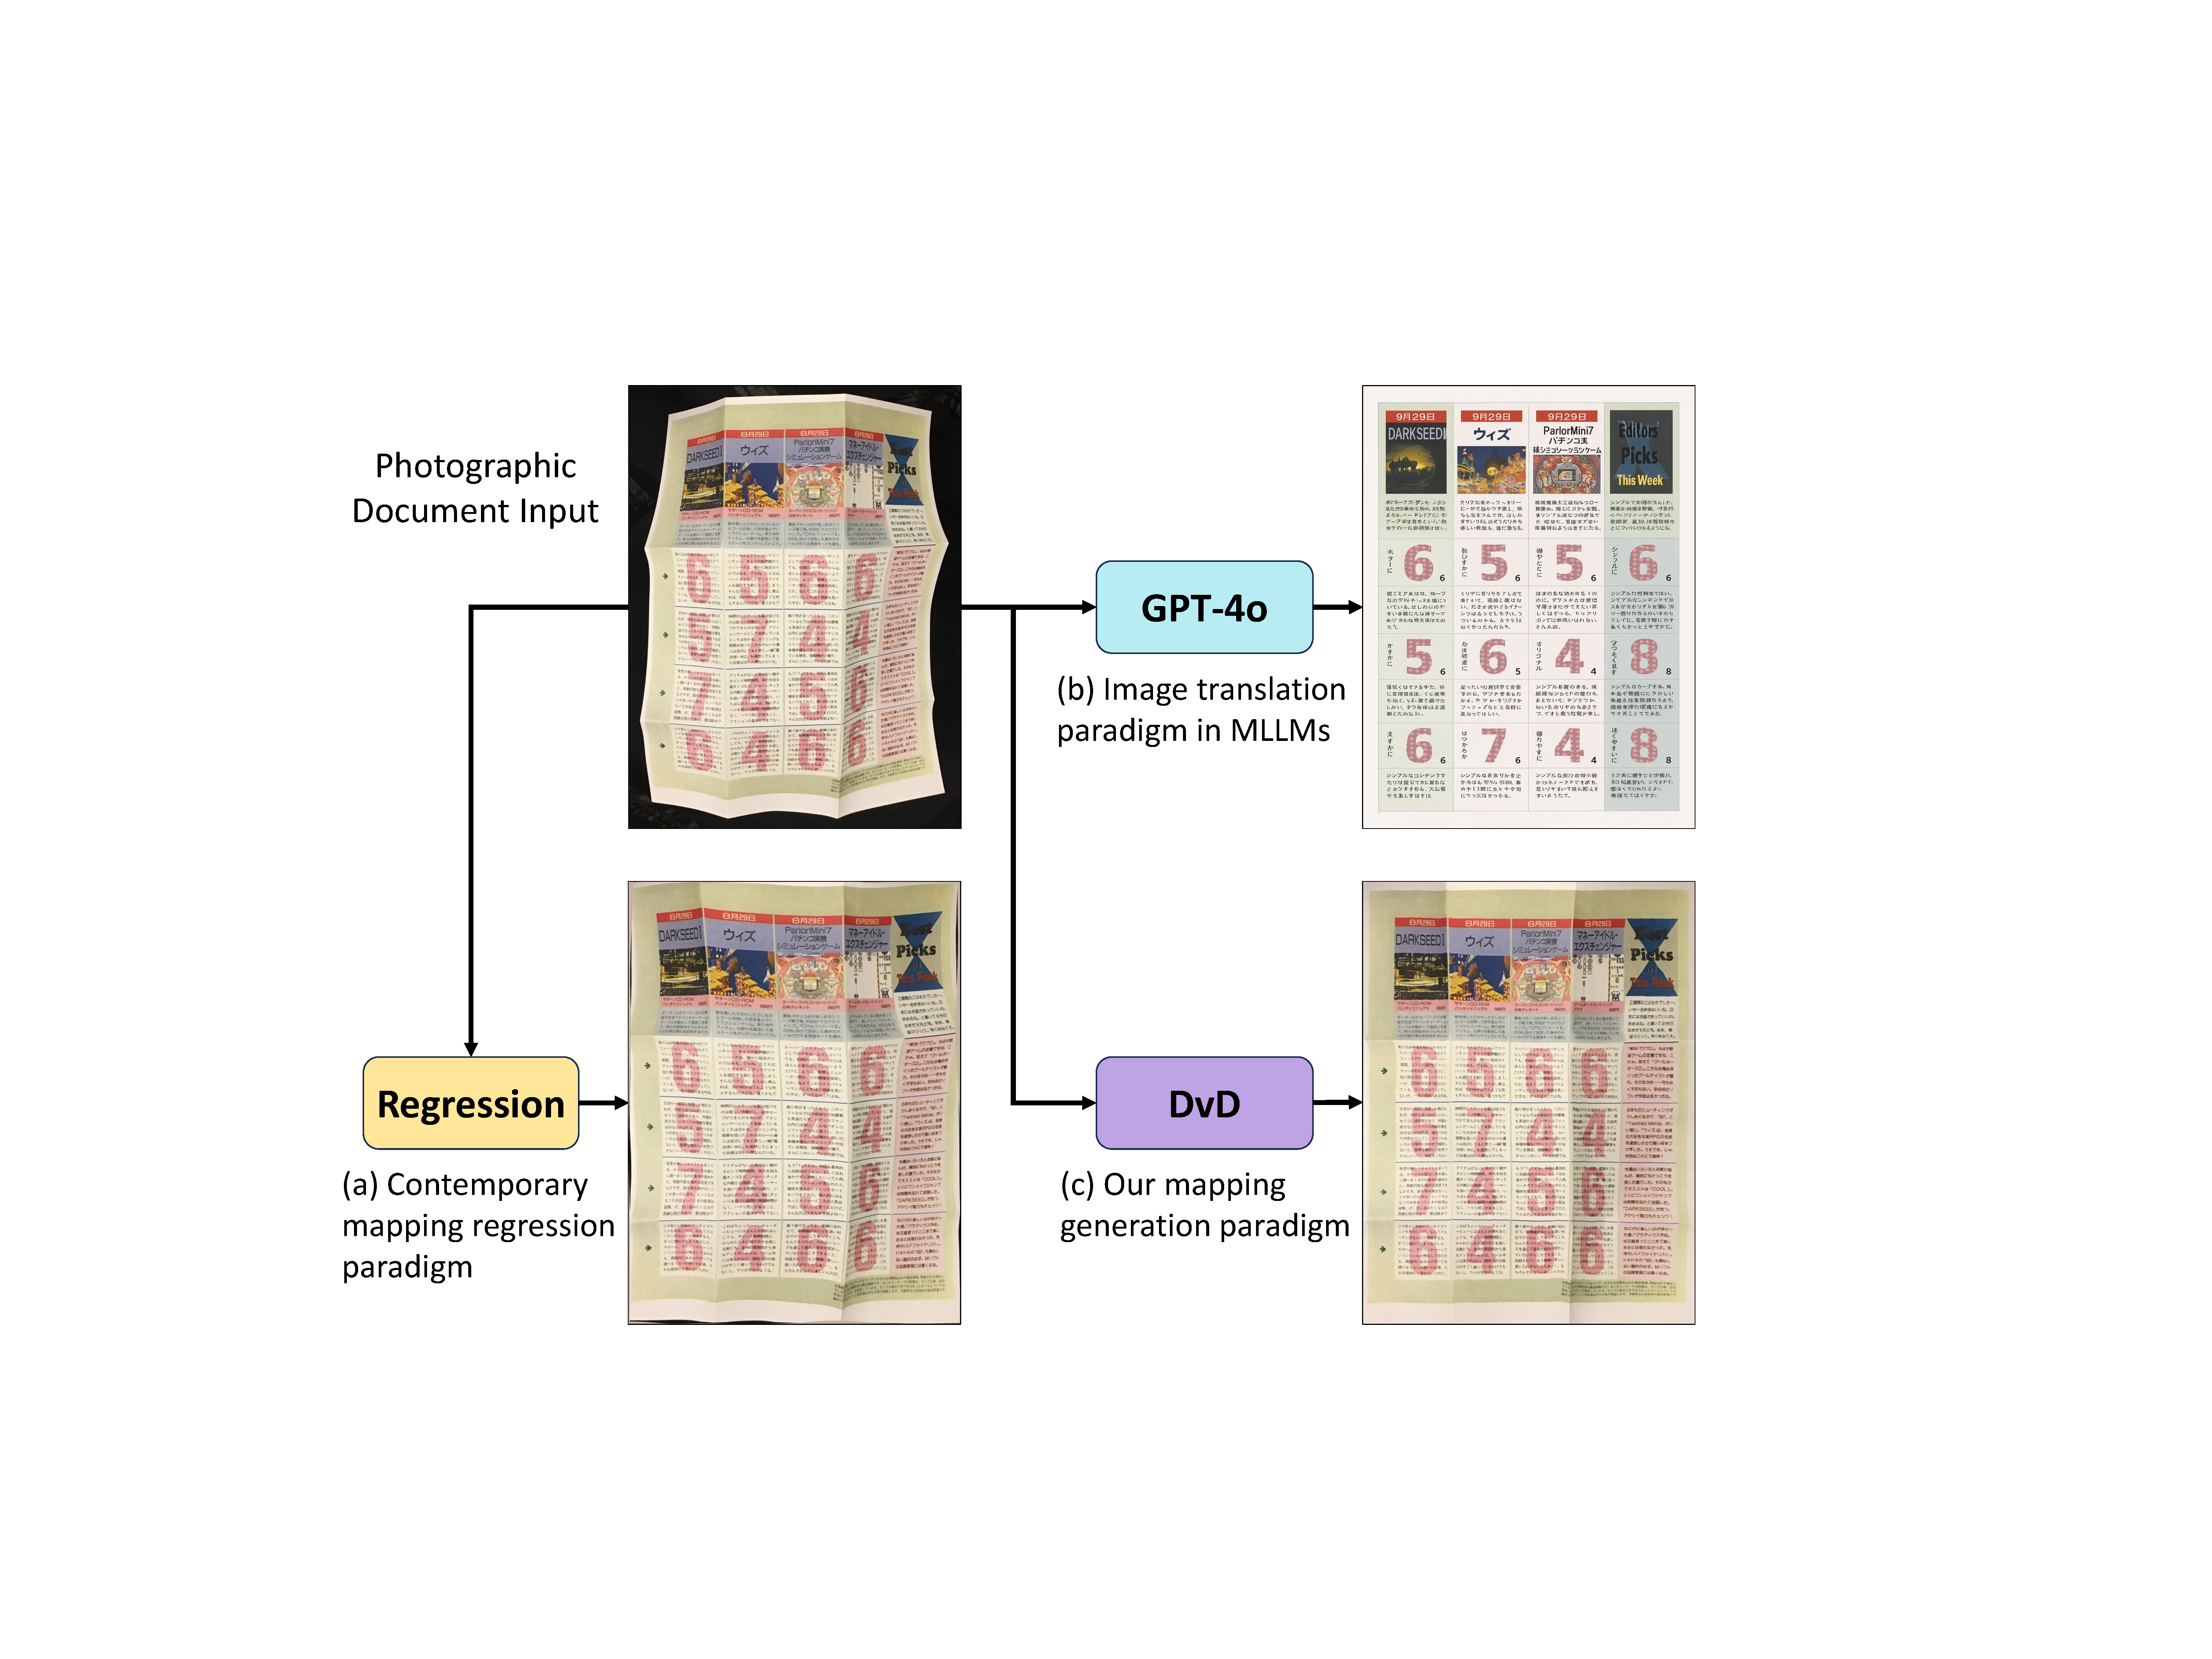
\includegraphics[width=\linewidth]{figures/head5.pdf}
	\caption{Comparisons to the existing paradigm for document
dewarping. Unlike the existing paradigms (a) and (b) struggle with either precise structural preservation or faithful content generation, our DVD (c) can yield flat document images with precise yet faithful content through a mapping generation paradigm.
}
\label{fig:head_img}
\end{figure} 
% but also pose substantial challenges
% and better generalization to real world.
% \textbf{Document image dewarping.}  (a) is an input warped document. (b$\sim$d) is dewarped results from (b) DocGeoNet~\cite{Feng2022geodocnet}, (c) FTA~\cite{li2023foreground}, (d) Our work. (e) is a ground truth flat document for reference.
% For better comparison, we provide anaglyphs (b'$\sim$d') that illustrate the large spatial misalignment between dewarped (b$\sim$d) and flat document (e), denoted as \textbf{"$\boldsymbol{\oplus}$"}. We highlight some conspicuously misaligned regions by dotted lines. Compared with previous state-of-the-arts, our DvD performs less content misalignment and ensures foreground integrity.



% emerging as a meaningful task over the past three decades~\cite{Kanungo_1993, li2023ladoc, yu_docreal_2024}


% To solve this issue, document dewarping has emerged as a meaningful task over the past three decades~\cite{Kanungo_1993, li2023ladoc, yu_docreal_2024}, restoring flat documents to benefit downstream document digitization tasks~\cite{li2025docsam, wan_2024_multidetect}. 


% 第二段：回顾当前方法主要在贡献数据和网络结构来改进
Document dewarping has evolved through two distinct periods. The early model-based methods~\cite{Kanungo_1993, cao2003cylindrical, RN19} basically follow a "reconstruct-then-dewarp" paradigm, which is typically limited by hardware dependence or surface assumptions.
Subsequent data-driven methods~\cite{ma2018docunet, li2019document, das2019dewarpnet} have shifted toward a mapping regression paradigm to model the condition probability. Specifically, given a large-scale photographic document dataset, these methods predominantly train neural networks to directly regress mapping (e.g., backward mapping, forward mapping) for dewarping. Accordingly, they also transfer the research attention to high-fidelity training data~\cite{zhang_2024_docregistration, verhoeven2023neural, zhang2024reg} and better network architecture for feature extraction~\cite{li2023foreground, Feng2022geodocnet}. 

% 第三段 当前问题：矫正结构保持不好(果)->判别式模型的分布学习能力不好(因)；
% 当前现状，扩散模型很好，但是无法直接应用于文档矫正
Albeit accomplishing notable advancements, the contemporary mapping regression paradigm is burdened by its intrinsic discriminative nature, which lacks the capacity to explicitly capture the underlying data distribution, resulting in imprecise structural preservation (See Fig.~\ref{fig:head_img} (a)).
Recent diffusion models have demonstrated the viability of employing a generative paradigm to solve discriminative tasks~\cite{ravishankar_2024_scaling, nam_2024_diffmatch, luo2024flowdiffuser}. By learning a progressive denoising process to generate samples conforming to the training data distribution, these models introduce a generative task modeling to learn more comprehensive distributions.
Most recently, MLLMs (e.g., Gemini 2.5, GPT-4o) have exhibited remarkable natural image generation capabilities~\cite{yan2025gpt-imgeval}, but failed to preserve document structures in document dewarping (e.g., Fig.~\ref{fig:head_img} (b)). We attribute this to the fact that it’s very difficult to directly employ an image translation
paradigm to obtain faithful control in highly complex document images. In light of these insights, we propose one intriguing question: \textit{Can generative models be effective for document dewarping?}


%####################################################
%  but it is still challenging to preserve document structures. Given recent advances in diffusion models, it is natural for us to consider their potential applicability to document dewarping. However, it is far from straightforward to adopt diffusion models in document dewarping due to their unfaithful control on high-resolution document images (e.g., 2000×3000). 

% has commonly been approached by a mapping regression paradigm in the age of deep learning. 
%Despite notable advancements, their intrinsic discriminative nature lacks the capacity to explicitly capture the underlying mapping distribution, resulting in imprecise structural preservation.
%On the other hand, generative models, epitomized by diffusion models, are proficient in capturing more comprehensive probability distributions and thus provide a promising solution; however, their high computational cost (e.g., 2000$\times$3000 resolution) and unfaithful controllability limit their feasibility.
%####################################################



% 第四段: 如何在矫正任务应用diffusion的多步任务建模
% 坐标空间形变建模+TVCR=好的矫正结构保持能力
To answer this question, we present DvD, the first effort to unleash a generative dewarping model built on a coordinates-based denoising diffusion framework. Instead of typical pixel-level denoising, we introduce a coordinate-level denoising process, where DvD learns how to progressively generate a series of latent variables to characterize the mapping for deformation rectification. We argue that such a mapping generation paradigm not only explicitly fosters deformation-aware modeling but also avoids the difficulty of high-resolution image generation. 
To further enhance the structural preservation, DvD also incorporates a time-variant condition refinement mechanism to leverage intermediate dewarping results. Diverging from typical diffusion models guided by a time-fixed condition, our proposed time-variant mechanism enables intermediate-aware dynamic guidance in the denoising generation process.

 
% Guided by single warped document images
% We also give a theoretical analysis from the optimization perspective of condition likelihood.
% Unconventionally, moving beyond the previous discriminative paradigm, this paper pioneers a preliminary investigation on \textit{whether the generative paradigm is a more efficacious learning paradigm for document dewarping task.} To this end, we develop DvD, the first generative dewarping model built on a conditional denoising diffusion probabilistic framework. Guided by single warped document images, DvD learns how to progressively generate mapping through a reverse denoising process, rather than directly regression in a discriminative manner. To thoroughly delve into the potential of DvD in document dewarping, we systematically investigate three desirable properties of diffusion models and corresponding task-specific adaptability, as follows. 
% \textbf{(1) Denoising generation fosters better accuracy}: Instead of directly conditional probabilities modeling in discriminative paradigms, DvD fosters a more elaborate task modeling through denoising generation, yielding less content misalignment (See Fig.~\ref{fig:head_img}). For one thing, DvD introduces a series of latent variables to progressively model the conditional likelihood. For another thing, inspired by hand-crafted multi-stage models~\cite{jiaxin2022marior, yu_docreal_2024}, DvD incorporates a time-variant condition refinement mechanism tailored for leveraging intermediate dewarping results. We also give a theoretical analysis from the optimization of condition likelihood. See Sect.~\ref{sec:method31}, \ref{sec:method33}.


% new 第五段 fine-grained dewarping evaluation
To make the evaluation of dewarping models fairly, we collect most of publicly available document dewarping benchmarks as shown in  Table~\ref{tab:unwarping_datasets}. We find that these benchmarks typically suffer from three critical limitations that impede a comprehensive evaluation of dewarping models, including restricted coverage of real-world scenarios, a small dataset scale, and deficient annotation of domains. 
These limitations might have led to evaluation ambiguity, restricting the model's application in real-world scenarios. To this end, we construct a fine-grained and large-scale benchmark AnyPhotoDoc6300, which contains 6,300 real-world photographic image document pairs, rigorously organized across three distinct domains, enabling fine-grained evaluation of dewarping models. In addition to the benchmark, we extend the evaluation metrics. We find that existing methods commonly utilize off-the-shelf OCR engines to measure the Edit Distance (ED) and Character Error Rate (CER) as OCR metrics~\cite {das2019dewarpnet}. 
We identify that there is still no exploration about whether the dewarped document can attain equivalent text readability to its flat counterpart for MLLMs.
To fill the blank, we propose two MLLM-based OCR metrics (MMCER and MMED) in this work. 



% We identify that there is no exploration about whether document dewarping is still useful for OCR using MLLMs. 
% We identify that there is still no exploration about the extent to which dewarped documents can enhance text readability in MLLMs.

% , none of the benchmarks enable fine-grained dewarping evaluation in the real world. 
% most benchmarks either focus on certain scenarios or roughly mix samples from multiple scenarios.
% Particularly, DocReal~\cite{yu_docreal_2024} and Inv3DReal~\cite{hertlein2023inv3d} focus on specific scenarios (i.e., invoices and Chinese documents).
% UVDoc~\cite{verhoeven2023neural} adopts synthetic documents to moderate domain entanglement caused by environmental lighting variations.
% DocUNet~\cite{ma2018docunet} and DIR300~\cite{Feng2022geodocnet} coarsely mix hundreds of documents from multiple scenarios without distinguishing domains explicitly, constituting inherent domain entanglement.
% Although DocUNet and DIR300 remain the most widely used benchmarks for document dewarping, their severe domain entanglement introduces evaluation ambiguity, fundamentally limiting their utility for more elaborate analysis (e.g., generalization assessment). 







% 第六段 after=\vspace{-0pt}
In summary, our main contributions are four-fold:
\begin{itemize}[topsep=1pt,leftmargin=*] 
\item Pioneering a paradigm shift, we present DvD, the first generative model to tackle document dewarping via a coordinates-based diffusion framework. Unlike typical pixel-level denoising to generate dewarped images directly, we operate coordinate-level denoising to generate coordinate mappings for dewarping.
\item We introduce a time-variant condition refinement mechanism that dynamically leverages intermediate dewarping results as guidance to enhance the preservation of document structures. 
\item To offer a comprehensive evaluation of document dewarping models, we construct a fine-grained benchmark dataset AnyPhotoDoc 6300, which contains 6,300 real-world photographic image document pairs, rigorously organized across three distinct domains.
\item Extensive experiments demonstrate state-of-the-art dewarping performance with acceptable computational efficiency. 
\end{itemize}


\begin{table}[t]
\centering
\caption{Comparison of document dewarping benchmarks. \ding{55} symbolizes that this benchmark doesn't explicitly distinguish this domain. \textbf{Scenes:} Multiple scenarios (Mul), Real (R), Synthetic (S). \textbf{Domains:} Layouts Category (L), Environment Lighting (E), Capture Angles (A). }
\label{tab:unwarping_datasets}
\resizebox{\linewidth}{!}{
\begin{tabular}{lccccc}
\toprule
\multirow{2.5}{*}{\textbf{Dataset}} &\multirow{2.5}{*}{\textbf{Scenes}} &\multirow{2.5}{*}{\textbf{Images}} &\multicolumn{3}{c}{\textbf{Domains}} \\
\cmidrule(lr){4-6}
 & & &\textbf{L} &\textbf{E} &\textbf{A}\\
\midrule
DocUNet~\cite{ma2018docunet} &Mul-R &$130\times2$  &\ding{55}  &\ding{55} &\ding{55}\\             
DIR300~\cite{Feng2022geodocnet}  &Mul-R &$300\times2$    &\ding{55}  &\ding{55} &\ding{55}\\
Inv3DReal~\cite{hertlein2023inv3d} &Invoice-R  &$360\times2$    &1  &3 &1\\
UVDoc~\cite{verhoeven2023neural} &Mul-S &$50\times2$ &\ding{55} &\ding{55} &\ding{55}\\
DocReal~\cite{yu_docreal_2024} &Chinese-R  &$200\times2$    &\ding{55}  &\ding{55} &\ding{55}\\
\textbf{Our AnyPhotoDoc6300} &\textbf{Mul-R} &$\textbf{6300}\times2$  &\textbf{8}  &\textbf{3} &\textbf{2}\\
\bottomrule
\multicolumn{6}{l}{\small $\bullet$ Noted that we don't list WarpDoc~\cite{xue2022fourier} and SP~\cite{li2023ladoc} }\\ 
\multicolumn{6}{l}{ due to open-source incompleteness.}
\end{tabular}}
\end{table}






% \textbf{Firstly}, single-step task modeling is overly simplistic to perceive subtle deformations. Therefore, existing methods fail to achieve precise structural preservation for document content and even bring in extra artifacts (See Fig.~\ref{fig:head_img} (a)), ultimately resulting in suboptimal regression precision.
% \textbf{Secondly}, the regression networks commonly adopted by prevalent methods fundamentally belong to discriminative models, which lack the capability to explicitly capture the underlying probability distribution that characterizes the dense mappings, consequently hampering their generalization in real-world scenarios.

% their intrinsic single-step discriminative nature.
% In contrast to discriminative paradigms that directly regress mapping or mapping,
% Instead of directly conditional probabilities modeling in discriminative paradigms
% While they superficially produce flattened and clean outputs, the absence of deformation modeling leads to missing and erroneous document contents.
% such as depth estimation~\cite{ravishankar_2024_scaling}, image matching~\cite{nam_2024_diffmatch}, semantic segmentation~\cite{ji_ddp_2023}, and optical flow estimation~\cite{luo2024flowdiffuser} achieving success across multiple dense prediction tasks


% To improve the regression accuracy, they primarily pursue three directions: the contribution of high-fidelity photographic document datasets or the advancement of document representation learning through enhanced visual feature extraction architectures and more sophisticated neural network designs.

% These methods typically rely on special hardware or surface assumptions to obtain a 3D reconstruction, followed by hand-crafted transformations for flattening documents to the plane.
% However, such assumptions lead to limited generalization in real scenarios, and the dependence on hardware deviates from the user habits of mobile-centric.
% significantly lessening reliance on both assumptions and hardware. 

% For instance, as shown in Fig.~\ref{fig:head_img} (b, b', c, c'), current state-of-the-arts 
% are still far from being applied in real-world scenarios, 

% including misaligned document content and redundant backgrounds,

% Subsequent learning-based methods bring a paradigm shift from model-driven to data-driven, with minimal dependence on both assumptions and hardware.
% The early model-based methods~\cite{cao2003cylindrical, RN19, RN17} either utilize strong assumptions to devise some kind of transformations with limited generalization to warping patterns in real-world, or rely on special hardware to capture point-wise 3D transformations in an assumption-free manner whereas deviating from the user habit of using mobile phones to digitalize documents.
% tradition , RN11 RN20
% Numerous efforts have been undertaken to address the document dewarping task using either traditional methods or learning-based methods.
% pioneered by Ma et al.~\cite{ma2018docunet},
% thereby quickly becoming a predominant paradigm.
% these methods could be categorized into two branches:  methods and learning-based methods. 

% Document dewarping has been extensively studied through two primary approaches: traditional methods and learning-based techniques (see Table~\ref{tab:tab1}). Early traditional methods~\cite{RN11, RN17, RN19, RN20} relied on strong scene assumptions to design hand-crafted geometric transformations. While effective in constrained scenarios, these methods exhibited limited generalization to real-world warping patterns. Alternative hardware-dependent solutions utilized 3D scanning devices to capture point-wise transformations in an assumption-free manner, but such approaches conflicted with the prevalent practice of document digitization using mobile cameras.
% In contrast, learning-based methods, pioneered by Ma et al.~\cite{ma2018docunet} in 2018 and further developed in~\cite{li2019document, das2019dewarpnet, RN7}, have emerged as the dominant paradigm due to their minimal reliance on explicit assumptions or specialized hardware. These methods typically adopt a discriminative approach based on pixel-wise regression, achieving state-of-the-art performance in recent works~\cite{RN58, verhoeven2023neural, li2023ladoc, yu_docreal_2024}. However, persistent challenges remain, including content misalignment artifacts and incomplete suppression of redundant backgrounds, as demonstrated in Fig.~\ref{fig:head_img} (b, b', c, c').

% In contrast to discriminative paradigms that directly regress mapping or mapping,

% To the best of our knowledge, it's the first attempt to formulate the task by generative paradigm, moving beyond the previous discriminative paradigm by three appealing properties. 

% In contrast to discriminative paradigms that directly regress mapping or mapping, DvD establishes a conditional denoising diffusion framework to tackle the task by learning how to generate mapping from Gaussian noise. 
% Building upon the recent success of diffusion models in visual computing tasks~\cite{ravishankar_2024_scaling,mou_diffeditor_2024}, we introduce a conditional denoising probabilistic  diffusion framework to serve as the core architecture of DvD.
% assert that the proposed generative paradigm shows appealing potential thanks to the following three desirable properties and corresponding .






% Additionally, we pioneer an exploration about whether document dewarping is still useful for OCR using multimodal large-language models(MLLMs), with proposed MMCER (MLLMs-based Character Error Rate) and MMED (MLLMs-based Edit Distance) serving as specialized supplements to previous OCR metrics.


% To address the issue, inspired by the rapid progress of recent MLLMs in OCR capabilities~\cite{wei2024general, nassar_smoldocling_2025}, we introduce replace traditional OCR engines with MLLM to measure OCR metrics (i.e.,~CER, ED). See Sect.~\ref{sec:metric}.

% Witnessing the superior progress of multimodal large language models (MLLMs) in OCR capabilities recently~\cite{wei2024general, karmanov_eclair_2025, nassar_smoldocling_2025}, we identify that there is no exploration about whether document dewarping is still useful for OCR using multimodal large-language models(MLLMs). To fill the blank

% Witnessing the rapid progress of multimodal large language models (MLLMs) in OCR capabilities recently~\cite{wei2024general, karmanov_eclair_2025, nassar_smoldocling_2025}, we introduce a pair of MLLM-based OCR metrics (i.e.,~MMCER, MMED) to replace the popular ED and CER.
% Specifically, we employ cutting-edge MLLM QWen2.5-VL~\cite{bai_2025_qwen25vl} to finish an image-to-markdown conversion task in both dewarped and flat documents, which assesses whether document dewarping task still improve text readability for MLLMs.
% We argue that OCR engines are neither robust nor versatile to different modality variations.

% 第四段：
% 基于上述吸引人的特性，我们还对香草扩散模型框架进行了延伸，使其更适合文档解翘曲任务。
% 两个方面。time-variant condition refinement mechanism + 后处理的样本筛选机制
% Building upon these appealing properties, DvD modifies the vanilla diffusion model through two task-specific improvements, making it more suitable for document dewarping. 
% For one thing, DvD incorporates an improved step-wise task modeling. We notice recent content-based iterative models treat dewarping as a multi-stage procedure, recursively feeding dewarped document content to a multi-stage model, which is proven to achieve visually pleasant alignment results(e.g., Marior~\cite{jiaxin2022marior}, DocReal~\cite{yu_docreal_2024}, and FDRNet~\cite{xue2022fourier}). Inspired by these successes, in DvD, we incorporate a time-variant condition refinement mechanism tailored for the training and sampling phase in the diffusion model, which holds two benefits for better optimization of condition likelihood. 
% (1) Compared with time-fixed conditions $y$, time-variant conditions $y_t$ can dynamically reduce Kullback-Leibler(KL) divergence in each diffusion time step, which thereby helps the model approach a tighter Evidence Lower Bound(ELBO)~\cite{pmlr-vae-2014}.
% (2) It can provide extra gradient compensation at each time step to mitigate the deviation of likelihood estimation caused by accumulated errors.

% 真~第五段
% Furthermore, we contribute a large-scale benchmark to fully evaluate our DvD. Existing document dewarping benchmarks either focus on coarse evaluation across hundreds of images (e.g., DocUNet~\cite{ma2018docunet} and DIR300~\cite{Feng2022geodocnet}) or specialized scene evaluation (e.g., Inv3DReal~\cite{hertlein2023inv3d}, DocReal~\cite{yu_docreal_2024}, LA-DocFlatten~\cite{li2023ladoc}, and UVDoc~\cite{verhoeven2023neural}), therefore providing limited evaluation ability. 
% To address their deficiencies in data scale (hundreds vs. our 7,000 pairs), dimensional coverage, and fairness, we construct AnyPhotoDoc7000 --- the largest comprehensive benchmark across five key dimensions: text density, warping patterns, lighting conditions, capture angles, and interfering factors. 
% To ensure fairness, we adopt a controlled-variable strategy by fixing text density dimensions to measure performance variations across the other four dimensions.






% 第五段原文
% Furthermore, most existing dewarping methods are evaluated on benchmarks such as DocUNet~\cite{ma2018docunet} and DIR300~\cite{Feng2022geodocnet}, which contain hundreds of real-world photographic document images across general scenarios. After that, several newer benchmarks (e.g., Inv3DReal~\cite{hertlein2023inv3d}, DocReal~\cite{yu_docreal_2024}, LA-DocFlatten~\cite{li2023ladoc}, and UVDoc~\cite{verhoeven2023neural}) have collected hundreds of images to assess document dewarping capabilities in specific scenarios. While these efforts are valuable, they exhibit limitations in dataset scale, evaluation fairness, and coverage of key dimensions. 
% To fill these lacks, we contribute AnyPhotoDoc, a comprehensive real-world document dewarping benchmark comprising 7,000 paired images designed for dewarping evaluation, with careful evaluation across five key dimensions: text density, warping patterns, environment lighting, capture angles, and interfering factors. To ensure fair and comprehensive multi-dimensional evaluation, we adopt a controlled-variable strategy by fixing text density dimensions to measure performance variations across the other four dimensions. As far as we know, AnyPhotoDoc is the largest and most comprehensive benchmark for document dewarping task up to now.

% 第六段原文
% Additionally, we further extend current OCR-based metrics in document dewarping. Because the primary goal of document dewarping is to enhance the readability of photographed documents, existing methods typically rely on OCR engines to evaluate improvements in text recognition performance. Witnessing the rapid progress of multimodal large language models (MLLMs) in OCR capabilities over recent years~\cite{Haotian_2023_llava, wei2024general, zhang_densetext_2024}, we propose a novel MLLM-driven OCR evaluation metric (including MMCER and MMED) to assess whether dewarped documents still improve text perception for state-of-the-art MLLMs. Specifically, we adopt the cutting-edge QWen2.5-VL~\cite{bai_2025_qwen25vl} as the evaluation model, instead of previous commercial OCR engines, to quantify the performance gap between dewarped documents and flat documents in image-to-Markdown conversion tasks.

% 具体地，DvD follows a conditional denoising diffusion framework to learn how to generate mapping for document dewarping, which allows diffusion training only in a smaller coordinate space, neatly bypassing the generation difficulties caused by high-resolution document images.
% Compared to previous discriminative models, 
% we explore the first generative model to revisit the document dewarping task. We introduce DvD, a simple yet effective diffusion probabilistic framework for 

% \item We revisit the document dewarping task and present DvD, which leverages a conditional denoising diffusion framework to progressively optimize likelihood from noise, capture multimodal distributions and enable robust stochastic sampling.
% To the best of our knowledge, it's the first attempt to employ a generative paradigm in document dewarping, moving beyond the previous discriminative paradigm.


% \item To further improve the learning of likelihood term, we introduce a time-variant condition refinement mechanism, leading to more precise alignment of document content with dynamic guidance. See Sect.~\ref{sec:method34}.
% \item We theoretically attribute the previous content iteration mechanism to the learning of likelihood term, and thereby introduce a time-variant condition refinement mechanism for diffusion model, leading to more precise alignment of document content. See Sect.~\ref{sec:method31}, \ref{sec:method33}.
% 通过更精细的条件信息，模型能更准确地捕捉条件对生成过程的约束，从而提升后验分布的似然估计。
% combined with a progressive mapping augmentation strategy
% which synergistically improves the vanilla diffusion model by enabling gradual learning of warping patterns and dynamic focus on details at each time step. 
% \item Furthermore, we introduce a progressive mapping strategy combined with a time-variant condition refinement mechanism to improve the vanilla diffusion model. This synergy helps the model to gradually learn the warping pattern at different time steps while dynamically focusing on different details based on time-variant conditions.

% \item We revisit the document dewarping task from a maximization of posterior probability formulation, critically analyzing the shortcomings of previous methods in either the likelihood term or the prior term. See Sect.~\ref{sec:method31}.
% \item Based on the formulation, we propose DvD, the first conditional diffusion framework tailored to jointly model both likelihood and prior terms. See Sect.~\ref{sec:method31}, \ref{sec:method32}.


% % 原段落5
% In particular, we initiatively present a probabilistic perspective explanation for the recent success of content-based iteration dewarping mechanisms that achieve visually pleasant alignment results(e.g., Marior~\cite{jiaxin2022marior}, DocReal~\cite{yu_docreal_2024}, and FDRNet~\cite{xue2022fourier}). These iterative models treat dewarping as a progressive process, recursively feeding dewarped document content to a multi-stage model, as illustrated in the last column of Tab.~\ref{tab:tab1}.
% % 对于扩散模型，我们将这种机制的成功解释为：通过更精细的条件更新，模型能更准确地捕捉条件对生成过程的约束，从而提升似然项的学习能力
% For diffusion models, we incorporate this mechanism as a time-variant condition refinement mechanism, which holds two benefits for the learning of condition likelihood.
% (1) Unlike time-fixed conditions, time-variant conditions can dynamically reduce Kullback-Leibler(KL) divergence in each diffusion time step, which in turn helps the model approach a tighter Evidence Lower Bound(ELBO)~\cite{pmlr-vae-2014}.
% (2) It can provide extra gradient compensation at each time step to mitigate the deviation of likelihood estimation caused by accumulated errors.












% we introduce DvD, the first conditional denoising diffusion framework to learn how to generate mapping for document dewarping. Unlike existing traditional or data-driven methods,
% DvD aims to explicitly learn the conditional posterior probability of mapping, which jointly models both likelihood and prior terms within the diffusion probabilistic process. Notably, our DvD performs the diffusion process in the coordinate space of the mapping, conditioned on the features of the warped document. 
% Compared with costly pixel space diffusion in most generative paradigms~\cite{ho_2020_ddpm, Cho_2024_CVPR, mou_diffeditor_2024}, 



% 原段落3
% From such a perspective, we summarize the modeling items of typical traditional methods and recent data-driven methods, as shown in Tab.~\ref{tab:tab1}. Traditional parametric methods primarily focus on defining hand-crafted prior terms, such as general cylindrical surface (GCS)~\cite{RN13,RN17,RN18}, or developable surfaces~\cite{RN19,RN11,Pilu_2001_cvpr}. Although these priors could help the model dewarp photographic documents in specific scenarios well (e.g.~unfolded book pages), they struggle to generalize across the diverse warping patterns in real-world scenarios. 
% Instead of explicitly modeling the prior term, recent learning-based methods~\cite{das2019dewarpnet, li2023foreground, Feng2022geodocnet, jiang2022RDGR} have shifted their attention to directly learning the likelihood term using deep neural networks. Despite achieving new state-of-the-art, they still face unsolved issues, including misaligned document content and redundant backgrounds, as shown in Fig.~\ref{fig:head_img} (b, b', c, c'). 
% We attribute this to their sole concentration on likelihood maximization while neglecting an explicit warping prior, thereby limiting their capability to learn the ideal manifold of mapping.



% and leading to misaligned document content and redundant background.
% They also argue that vast amounts of data could help models implicitly understand the manifold of mapping.

% despite over two decades of research, even
% Unlike them, recent approaches (Kim et al., 2017a; Sun et al., 2018; Rocco et al., 2017; 2020; Truong et al., 2020b; Min \& Cho, 2021; Kim et al., 2018; Jiang et al., 2021; Cho et al., 2021; 2022) have focused on solely learning the data term with deep neural networks. 
% However, despite demonstrating certain performance improvements, these methods still struggle with effectively addressing the inherent ambiguities encountered in dense correspondence, including challenges posed by textureless regions, repetitive patterns, large displacements, or noises. 

% Parametric models often rely on strong assumptions, such as general cylindrical surface (GCS)~\cite{RN13,RN17,RN18}, or developable surface~\cite{RN19,RN11}. Unfortunately, these strong assumptions limit the models to be used in special scenes.

% Since the deformation of paper essentially occurs in 3D space, a typical approach is to apply the estimation of the 3D shape of the warped document as prior information and then complete the subsequent dewarping. We call such an approach 3D shape-based dewarping, which can be further divided into parametric and non-parametric models.

% Parametric models often rely on strong assumptions, such as general cylindrical surface (GCS)~\cite{RN13}, or developable surface~\cite{RN19}. Unfortunately, these strong assumptions limit the models to be used in special scenes. 

% On the other hand, non-parameterized models are more suitable to handle highly diverse document deformation, as they abandon such assumptions and estimate accurate 3D representation directly, such as mesh~\cite{RN28} and Non-Uniform Rational B-Splines (NURBS)~\cite{RN25}, while their models demand hardware heavily, like multi-view imaging~\cite{RN25}, laser range scanner~\cite{RN29} and structured light~\cite{RN21}, which fall behind the pace with the popularity of mobile camera.

% We can't help but ask: \textbf{Can we propose a novel model to unify the likelihood term and the prior term?} 
% 原段落4
% Fortunately, recent diffusion models~\cite{ho_2020_ddpm, Alexander_2020_ddim, Song_2019_Generative} have demonstrated incredible ability to learn posterior probability, showing versatility in various vision tasks, such as image generation~\cite{mou_diffeditor_2024, Cho_2024_CVPR},  segmentation~\cite{ji_ddp_2023}, object detection~\cite{Chen_2023_ICCV}, depth estimation~\cite{ravishankar_2024_scaling}, image matching~\cite{nam_2023_diffmatch}, and optical flow estimation~\cite{Saxena_2023_optical}. Inspired by the success of these diffusion models, we introduce DvD, the first conditional denoising diffusion framework to learn how to generate mapping for document dewarping. Unlike existing traditional or data-driven methods, DvD aims to explicitly learn the conditional posterior probability of mapping, which jointly models both likelihood and prior terms within the diffusion probabilistic process. Notably, our DvD performs the diffusion process in the coordinate space of the mapping, conditioned on the features of the warped document. 
% Compared with costly pixel space diffusion in most generative paradigms~\cite{ho_2020_ddpm, Cho_2024_CVPR, mou_diffeditor_2024}, our framework allows training only in a smaller coordinate space, neatly bypassing the generation difficulties caused by high-resolution document images.

% Specifically, our DvD employs warped documents and their feature descriptors as conditions, performing forward and backward processes in the coordinate space of mapping. This enables the model to learn how to generate mapping based on given conditions.
% Compared with performing the diffusion process in the pixel space of warped documents, our framework allows training only in latent space, which neatly circumvents the generation difficulties caused by the excessive resolution of warped documents.

% DvD uses warped documents and their feature descriptors as conditions, performing the diffusion process directly in the coordinate space of the mapping. This enables the model to learn to generate mapping based on the given conditions. Unlike pixel-space diffusion, our approach operates in latent space, alleviating the challenges posed by the high resolution of warped documents.

% Unlike costly pixel-space diffusion, our framework operates in smaller coordinate space, neatly circumventing the generation difficulties caused by high-resolution warped documents.

% This enables the model to learn how to generate mapping based on given conditions.

% to achieve more precise dewarping alignment in document content, we incorporate a time-variant condition refinement mechanism in the training and sampling process of the vanilla diffusion model to dynamically adjust detail focus across diffusion steps.


% Furthermore, as illustrated in the last column of Tab.~\ref{tab:tab1},
% To further improve the learning of likelihood term, we notice 
% recent content iteration mechanisms proposed in document dewarping task (e.g., Marior~\cite{jiaxin2022marior}, DocReal~\cite{yu_docreal_2024}, FDRNet~\cite{xue2022fourier}) demonstrate visually pleasant alignment capability,
%  we introduce a time-variant condition refinement mechanism, leading to more precise alignment of document content with dynamic guidance. See Sect.~\ref{sec:method34}.










% In our practice, at each step of the training and sampling stage, the generated mapping and its dewarped document image are recursively fed as dynamic guidance for the next time step.

 % adjust condition constraints within the diffusion reverse process， 
% This mechanism enhances the training signal by stabilizing gradient updates and reducing the local Kullback-Leibler divergence at each diffusion step, which in turn tightens the variational lower bound. 

% dynamically adjusts condition constraints within the diffusion reverse process; 

% the model holds the potential to approach a tighter Evidence Lower Bound(ELBO), which 降低了每一扩散时间步的 KL 散度. 
% For the diffusion model, we explain the success of this mechanism as follows: through more refined condition updates, the model could more accurately capture the constraints of the conditions on the generation process, thereby improving the learning ability of the likelihood term.
% Diffusion models, with their inherent iterative denoising process, hold the potential for applying this mechanism to achieve more precise dewarping alignment in document content.
% To this end, we incorporate a novel time-variant condition refinement mechanism into the training and sampling algorithm of vanilla diffusion. 

% , enabling the model to refine the dewarping result in a coarse-to-fine manner. 
% we apply mapping generated at each diffusion time step and the corresponding dewarped document as the input for the next time step, creating time-dependent conditions that help the model dynamically focus on the current dewarping details at each step.


% Additionally, we introduce a novel data augmentation strategy called progressive mapping, which provides more diverse deformation patterns for the training data of warped documents at no extra cost.

% By combining the proposed training mechanism and data augmentation strategy, we drive the model to progressively learn to generate more refined mappings.

% to achieve more precise dewarping alignment in document content, we propose a time-variant condition refinement mechanism combined with a progressive mapping augmentation strategy to help the model dynamically adjust detail focus across diffusion steps for 

% which synergistically improves the vanilla diffusion model by enabling gradual learning of warping patterns and dynamic focus on details at each time step. 

% This synergy helps the model to gradually learn the warping pattern at different time steps while dynamically focusing on different details based on time-variant conditions.
% \setlist[enumerate,1]{label=(\Roman*)}


% improving both learning efficiency and the precision of the mapping prediction.

% , document dewarping has been widely studied but remains an unsolved task, 
% continuing to attract substantial attention due to its practical significance and unsatisfactory performance.

\begin{figure*}[ht]
	\centering
	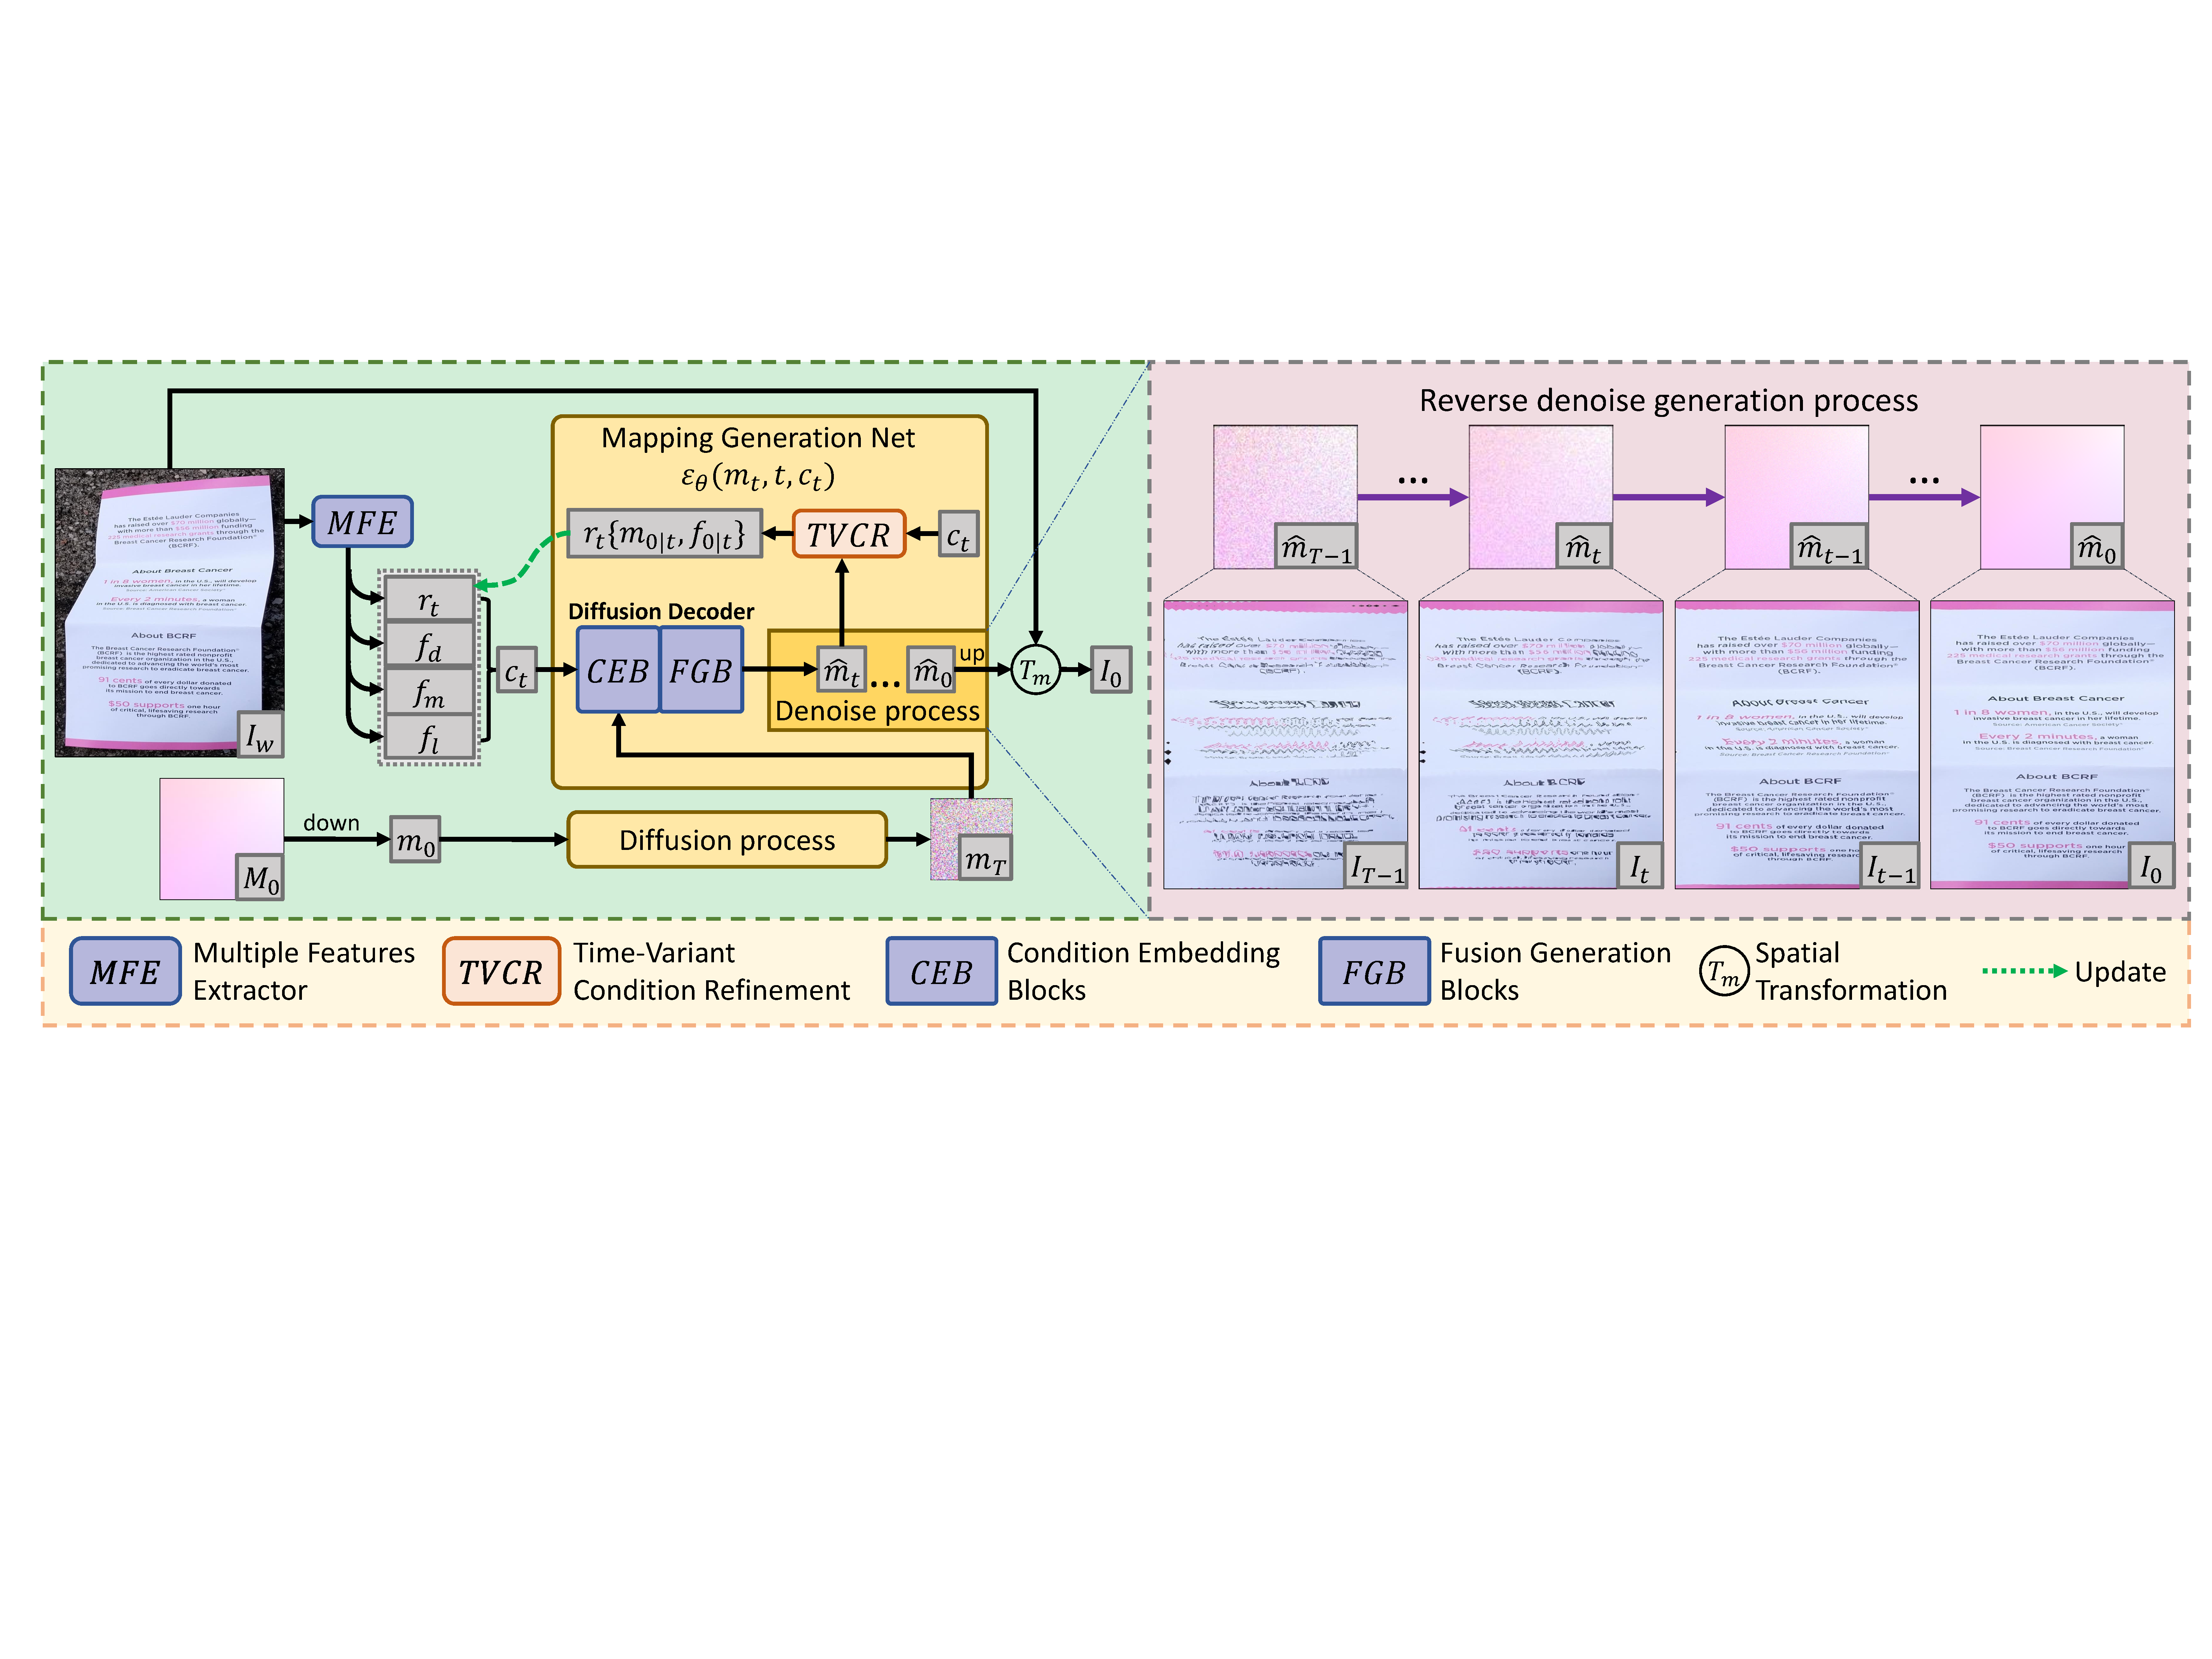
\includegraphics[width=\linewidth]{figures/fig2_v6.pdf}
	\caption{\textbf{Framework of the proposed DvD.} Given a warped document as input, DvD generates latent variables $m$ to characterize the mapping for deformation rectification. We leverage a compound condition $c_t$: the features for raw document images $f_d$, document foreground mask $f_m$, text-lines $f_l$, and the time-variant condition of the intermediate result $r_t$, respectively. We visualize the reverse denoise generation process in the right pink region.}
	\label{fig:img2}
\end{figure*}



\section{Related work}
\label{sec:related}
\subsection{Early Model-based Methods}
% Adhering to a two-step "reconstruct-then-dewarp" paradigm, % rely on special hardware or surface assumptions to obtain a document surface reconstruction, followed by hand-crafted transformations for dewarping the surface to the plane.
Early model-based methods basically adhere to a two-step "reconstruct-then-dewarp" paradigm. At the first step, for surface reconstruction, some methods utilize specialized hardware such as structured-light devices~\cite{RN26, RN21}, laser scanners~\cite{RN29}, multi-view camera systems~\cite{Ulges_2004, koo2009composition, RN11}, and proximal light sources~\cite{RN23}. Another methods bypass the hardware dependence by leveraging 2D visual cues (e.g., text lines~\cite{tian2011rectification}, local text orientation~\cite{RN18}, text blocks~\cite{RN16}, etc.) to estimate 3D geometry with parametric assumptions. 
In the second step, hand-crafted transformations for dewarping the surface to the plane are undertaken according to the reconstructed surface. For parameterized surfaces, typical transformations involve Generalized Cylinders Surface (GCS)~\cite{RN13, koo2009composition}, developable surfaces~\cite{RN19}, generalized ruled surfaces~\cite{Tsoi_2007}, and Non-Uniform Rational B-Splines (NURBS)~\cite{tan2005restoring}. For non-parameterized surfaces, techniques such as planar strips~\cite{RN20}, stiff mass-spring systems~\cite{RN29}, conformal mapping~\cite{RN11}, and sparse correspondence~\cite{RN18} are harnessed to tackle the mesh representation.
While effective in limited scenarios, these methods exhibited poor generalization to real-world warping patterns due to confined assumptions. Meanwhile, demanding hardware-dependent solutions also deviates from the prevalent habit of using mobile phones to digitize documents.



\subsection{Data-driven Methods}
Data-driven methods bring a shift toward a regression-based paradigm, significantly lessening reliance on both assumptions and hardware. Ma et al.~\citeyearpar{ma2018docunet} pioneer the application of deep neural networks to solve document dewarping by framing it as a mapping regression task. Subsequent DewarpNet~\cite{das2019dewarpnet} reformulates the traditional "reconstruct-then-dewarp" paradigm via two regression networks while collecting a high-quality synthetic dataset Doc3D using rendering software. CREASE~\cite{markovitz2020can} explores multi-modal warped document representations to strengthen the dewarping performance.
DocProj~\cite{li2019document} and PW-DewarpNet~\cite{das2021end} opt to dewarp documents in a patch-wise manner, benefiting the results at local details. DispFlow~\cite{xie2020dewarping} and DDCP~\cite{xie2021document} investigate the effectiveness of mapping and sparse control points as deformation representations, respectively. DocTr~\cite{feng2021doctr} replaces the convolutional network with a vision transformer, achieving significant performance boosts. 
RDGR~\cite{jiang2022RDGR}, DocGeoNet~\cite{Feng2022geodocnet}, and FTA~\cite{li2023foreground} leverage text-line features to keep textual content alignment. PaperEdge~\cite{RN58}, Marior~\cite{jiaxin2022marior}, and DocReal~\cite{yu_docreal_2024} devise two-stage networks, which first coarsely dewarp the mask of document, then refine details. 
FDRNet~\cite{xue2022fourier} introduces frequency-domain insight, designing an image-level loss based on high-frequency textures extracted from the Fourier transformation. UVDoc~\cite{verhoeven2023neural} exploits a novel data annotation pipeline through optical invisibility of ultraviolet ink to acquire pseudo-real training data. LA-Doc~\cite{li2023ladoc} constructs a synthetic dataset with large-scale deformation patterns via physical mass-spring systems and proposes a layout-aware dewarping network. Inv3D and DocMatcher~\cite{hertlein2025docmatcher,hertlein2023inv3d} present a template-based document dewarping using auxiliary template information. DocHFormer~\cite{zhou_dochformer_2025} introduces a novel shuffle transformer block to harmonize feature representation. DocRes~\cite{zhang_2024_docres} develops a unified model that integrates multiple low-quality document enhancement tasks. These methods concentrate on curating training datasets and devising regression networks, whereas their intrinsic discriminative nature is unexplored, which constrains the dewarping performance.

% (i,j)&=T_{m}(u,v)=F_0(u,v)+G(u,v),\\
\section{Methodology}
\label{sec:method}

%\subsection{Generative Task Modeling}
%\label{sec:method31}
%Unlike general image generation tasks (e.g., image editing), document dewarping requires not only precise structural preservation for document content but also high-resolution full-page documents. 
%Therefore, it's challenging to directly employ an image translation paradigm to model the task. To address this, we construct a mapping generation paradigm to explicitly foster a deformation-aware task modeling within the framework of the coordinate-based diffusion model, as shown in Fig.~\ref{fig:img2}. Specifically, we elaborate our method from four aspects below.

\begin{figure}[tp]
	\centering
	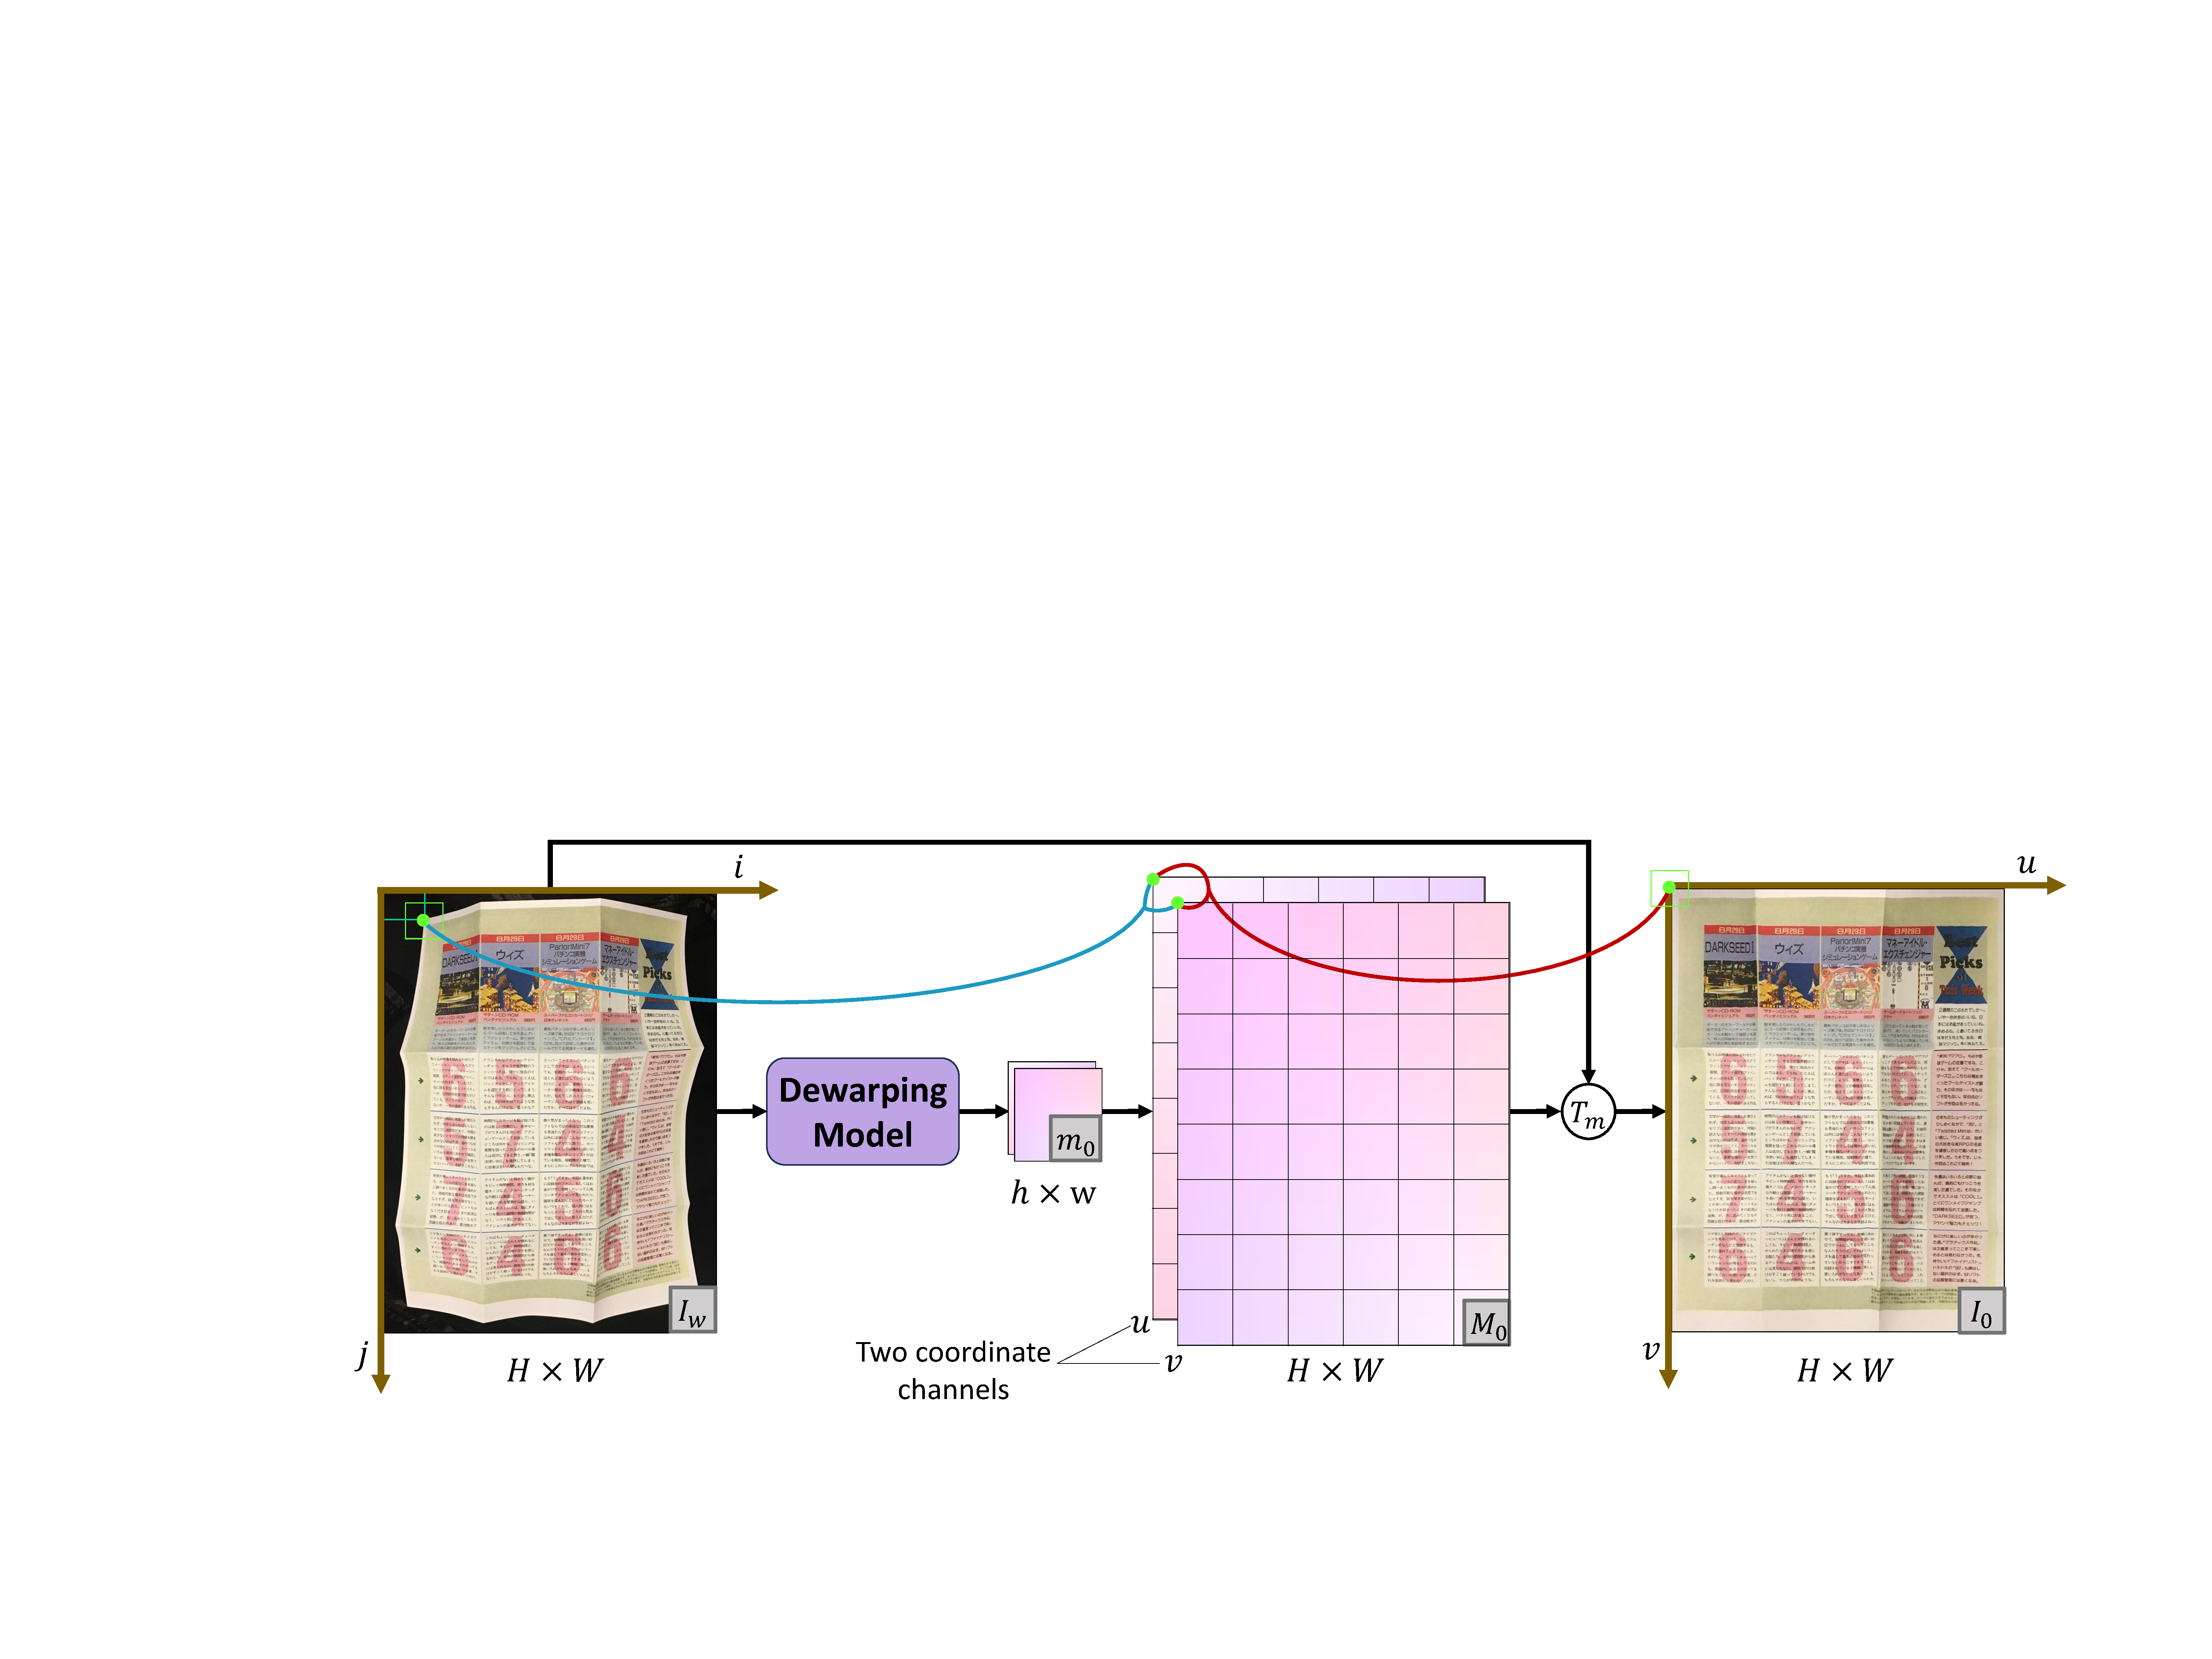
\includegraphics[width=\linewidth]{figures/fig_dewarp.pdf}
	\caption{General document dewarping pipeline. We propose a dewarping model to predict a backward mapping for deformation rectification, consisting of two coordinates channels.}
\label{fig:head_dewarp}
\vspace{-10pt}
\end{figure} 


\subsection{Document Dewarping Framework}
\label{sec:Framework}
As illustrated in Fig.~\ref{fig:head_dewarp}, given a warped photographic document image $I_w\in \mathbb{R}^{H\times W\times 3}$ as input, document dewarping aims to restore the flat document texture $I_0\in \mathbb{R}^{H\times W\times 3}$. In this work, we firstly propose a dewarping model to predict a small-scale coordinates mapping $m_0$, saving computational cost, which is then up-sampled to a normal backward mapping $M_0\in \mathbb{R}^{H\times W\times 2}$ (each value in $M_0$ represents the corresponding 2D coordinates in the input warped image $I_w$ as shown in Equ.~\ref{eq:def}), Next, we employ a dense spatial transformation $T_{m}$ to calculate the pixel values in $I_w$ according to the coordinates from $M_0$, ultimately obtaining $I_0$ as shown in Equ.~\ref{eq:def}. 
%Instead of directly generating $I_0$, we generate the backward mapping $M_0\in \mathbb{R}^{H\times W\times 2}$ (each value in $M_0$ represents the 2D coordinates of the pixels in the warped image $I_w$).
%Subsequently, we employ a dense spatial transformation $T_{m}$ to sample the pixels in $I_w$ according to the coordinates from $M_0$, ultimately deriving $I_0$. 
We formalize the backward mapping procedure as
\begin{equation}
\label{eq:def}
\begin{split}
(i,j)&=M_0(u,v),\\
I_0 (u,v)&= T_{m}(I_w(i,j)),
\end{split}
\end{equation}
where $(i,j)$ and $(u,v)$ represent the 2D spatial coordinates of $I_w$ and $I_0$, respectively. In the following, we will describe our dewarping model in details.


% which can explicitly depict the pixel-wise 2D deformation relationship between $I_w$ and $I_0$.


\subsection{Coordinates-Based Diffusion Model}
\label{sec:method31}
\subsubsection{Latent Diffusion Model in Coordinate Space.}
Directly generating $M_0$ explicit foster deformation-aware modeling to achieve better structural preservation, however both $M_0$ and $I_0$ actually contain equally high-resolution (e.g., 2000×3000), leading to high computational complexity. Inspired by the latent diffusion model~\cite{rombach2021highresolution}, we implement the diffusion and denoising processes only in a smaller coordinate space (i.e., $64\times64$), significantly reducing the training and inference costs. Figure~\ref{fig:img2} shows the overall framework of our proposed DvD model. Concretely, guided by a compound condition $c_t$, our DvD progressively generates a series of latent variables $m$ from a random Gaussian distribution. This paradigm relies on a tailored conditional denoising diffusion probabilistic framework, which typically contains both forward and reverse processes~\cite{ho_2020_ddpm, Song_2019_Generative}. We define the forward diffusion process for mapping as the Gaussian transition, s.t. $q(m_{t} | m_{t-1}) :=\mathcal{N}(\sqrt{1-\beta_t}m_{t-1}, \beta_t \mathbf{I})$, where ${\beta_t}$ is a predefined variance schedule. The resulting latent variable $m_t$ can be formulated as:
\begin{equation}
\label{eq:forward}
m_t = \sqrt{\bar{\alpha}_t}m_0 + \sqrt{1 - \bar{\alpha}_t}z, \quad z \sim \mathcal{N}(\mathbf{0},\mathbf{I}),
\end{equation}
where $\bar{\alpha}_t=\prod_{i=1}^t\left(1-\beta_i\right)$, and $m_{0}$ is the ground-truth mapping. 
Afterward, following Nichol and Dhariwal~\citeyearpar{Alexander_2020_ddim}, we train a neural network $\mathcal{\epsilon}_{\theta}(\cdot)$ for the reverse denoising process, during which the initial latent variable ${m}_{T}$ is iteratively denoised following the sequence ${m}_{T-1}, {m}_{T-2}, \ldots, {m}_{0}$, as follows:
\begin{equation}
\begin{split}
\label{eq:reverse_ddim}
m_{t-1} = &\sqrt{\bar{\alpha}_{t-1}}\mathcal{\epsilon}_{\theta}(m_t, t, c_t) +\\
&\frac{\sqrt{1-\bar{\alpha}_{t-1}-\sigma_t^2}}{\sqrt{1-\bar{\alpha}_{t}}}\Bigl(m_{t} - 
\sqrt{\bar{\alpha}_{t}}\mathcal{\epsilon}_{\theta}(m_t, t,c_t)\Bigr) + \sigma_{t}z,
\end{split}
\end{equation}
where $\mathcal{\epsilon}_{\theta}(m_t, t, c_t)$ directly predicts the denoised mapping $\hat{m}_{0,t}$.

\begin{figure}[tp]
	\centering
	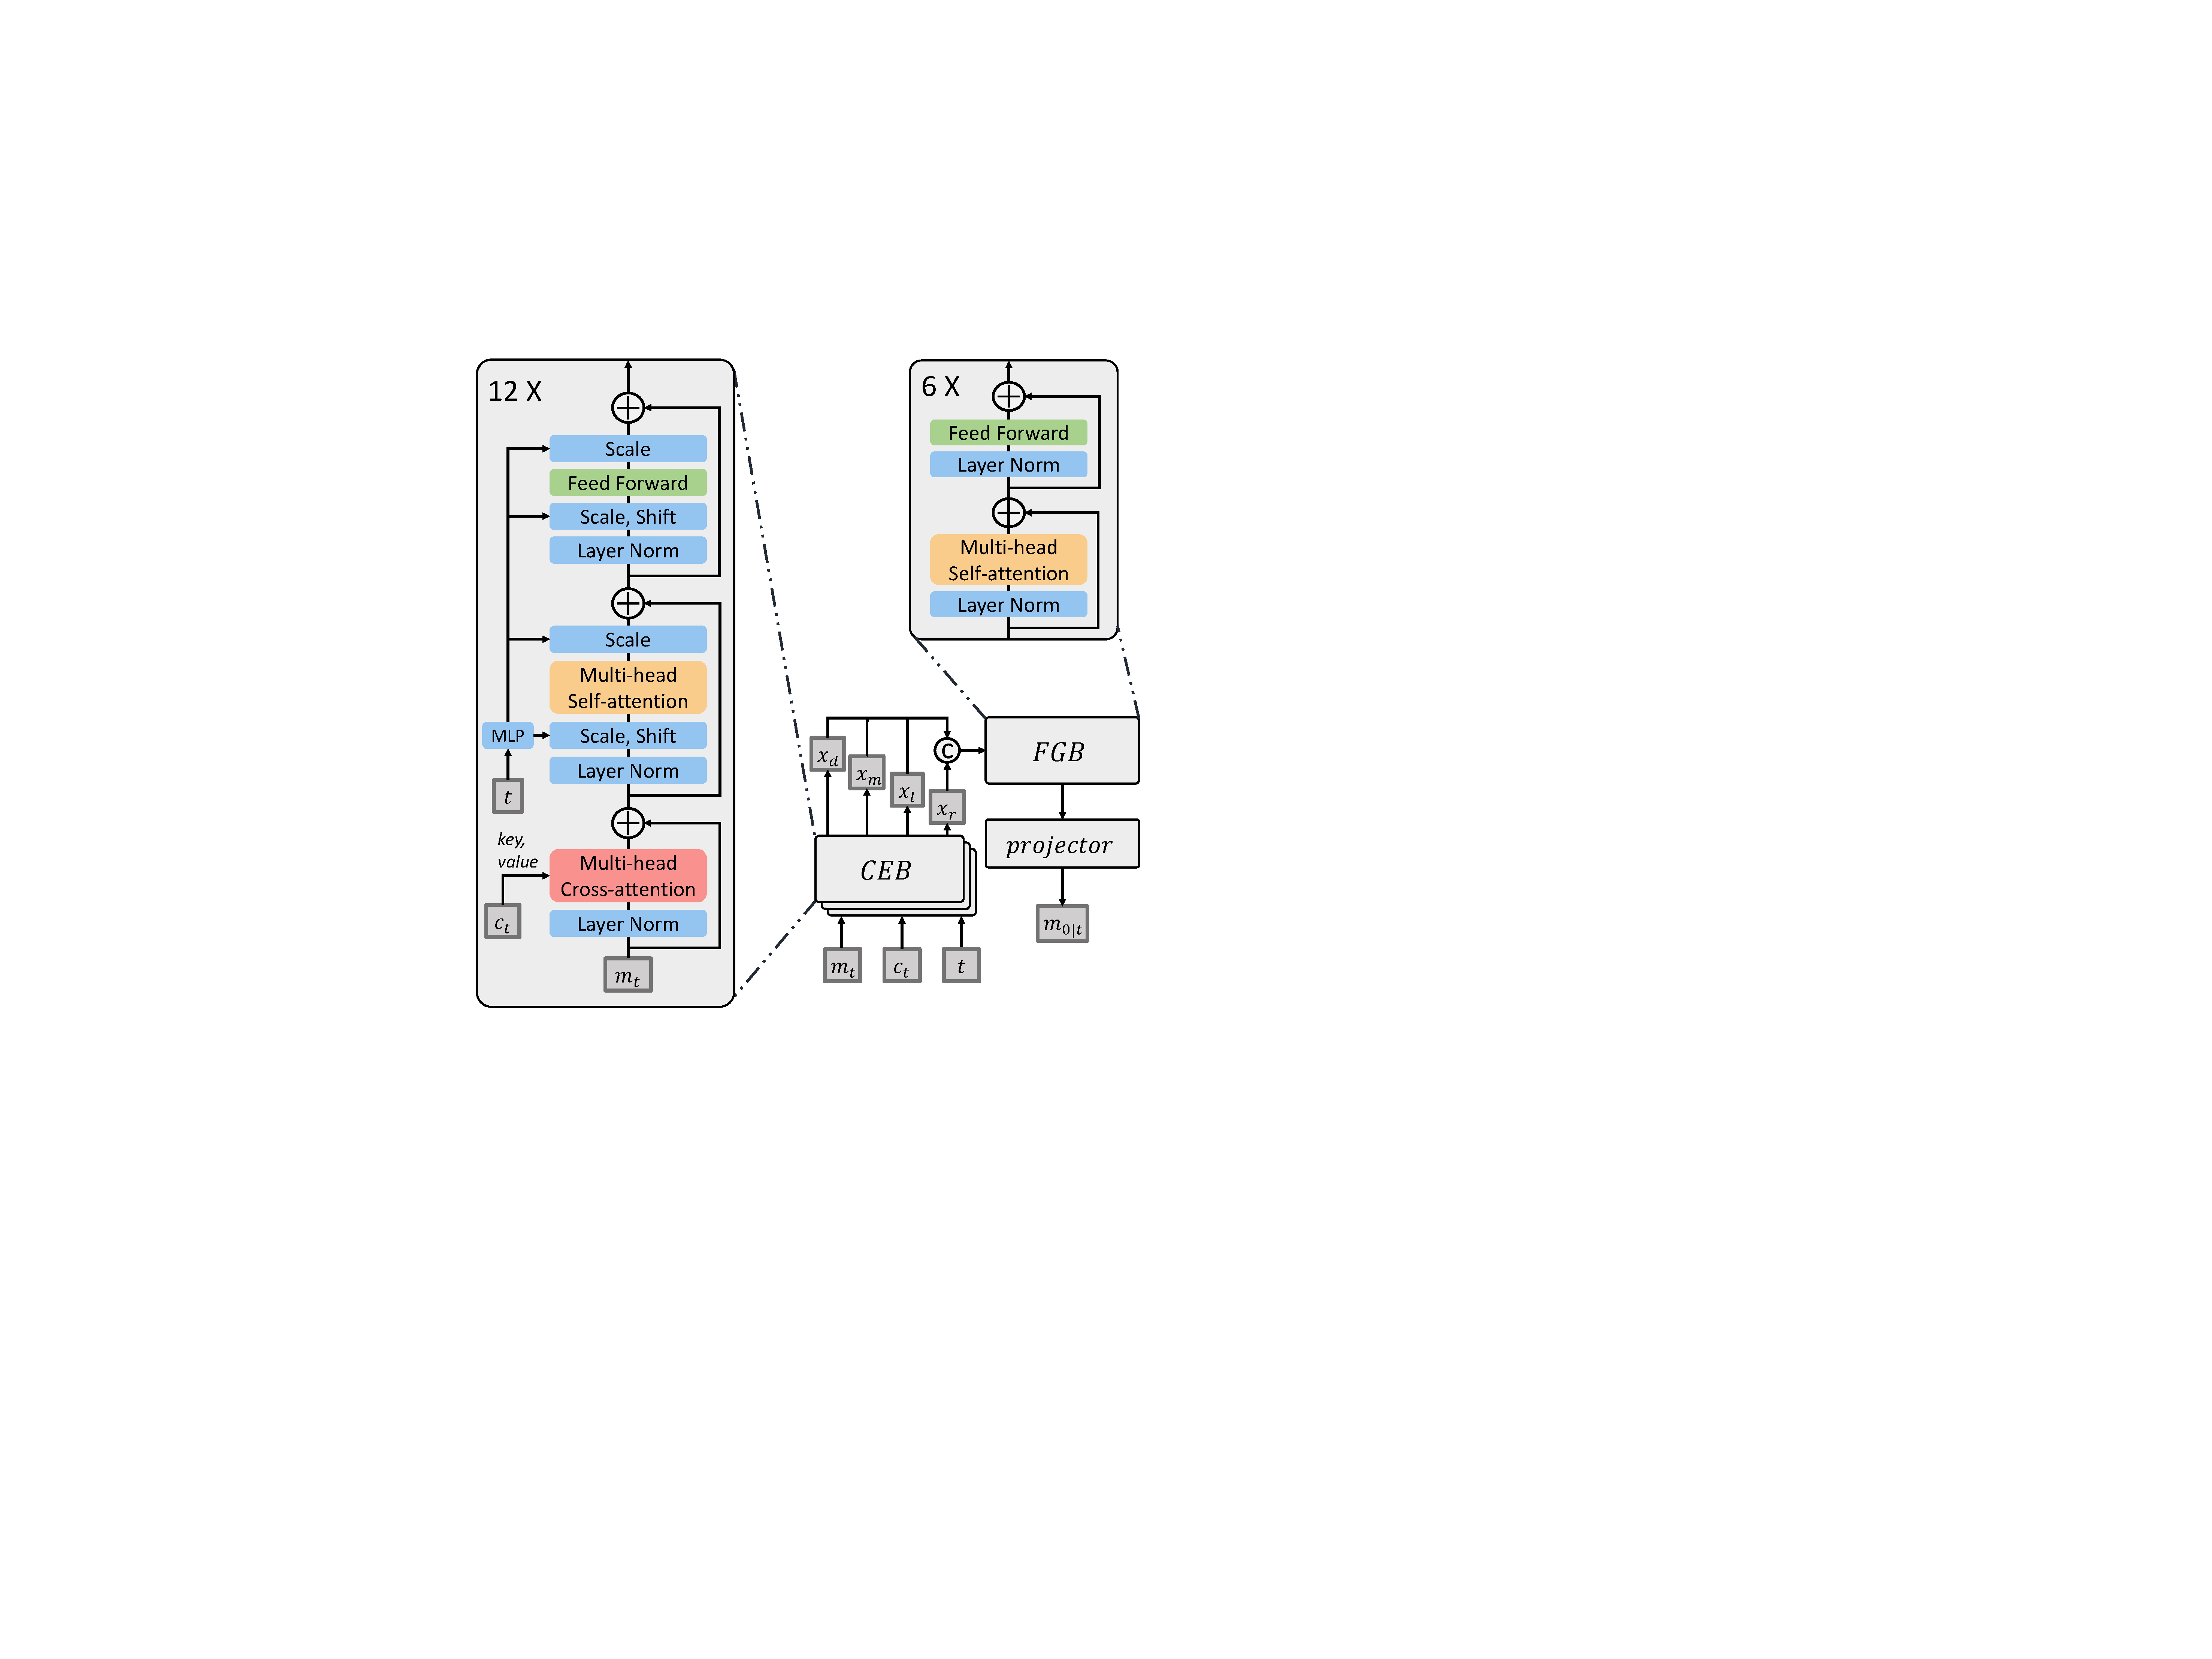
\includegraphics[width=0.9\linewidth]{figures/architect2.pdf}
	\caption{Detailed architectures of condition embedding blocks (CEB) and fusion generation blocks (FGB). We ignore some simple operations, such as cosine position encoding and activation functions.}
\label{fig:network}
\end{figure}

\subsubsection{Compound Conditions $c_t$.}
Following previous works~\cite{Feng2022geodocnet, li2023foreground, jiang2022RDGR}, our DvD utilizes pre-trained multiple feature extractors (MFE) to enhance document visual perception and composes these features into a compound condition for the diffusion model, denoted as $c_t=\{f_d, f_m, f_l, r_t\}$, where $f_d, f_m, f_l$ represent the features for raw document images, document foreground mask and text-lines, respectively. Note that $f_d,f_m,f_l$ are time-fixed conditions, while $r_t$ represents a time-variant condition that enables dynamic guidance in the denoising generation process. %We will elaborate on the time-variant condition in the next paragraph.

\subsubsection{Time-variant Condition Refinement (TVCR) Mechanism.}
% We observe that previous methods~\cite{jiaxin2022marior, yu_docreal_2024} adopt hand-designed multi-stage models to encourage coarse-to-fine structural preservation capability. 
As illustrated in the right region of Fig.~\ref{fig:img2}, the intermediate dewarping results reveal the visual gap from intermediate denoising states to the ideal dewarped result. To harness this information for enhanced preservation of document structures, we introduce a time-variant condition refinement mechanism within the reverse diffusion process to ensure increasingly precise document structure as the process evolves.
Specifically, we incorporate a time-variant condition $r_t=\{m_{0|t},f_{0|t}\}$ for iteratively updating $r_t$, where $m_{0|t}$ means the predicted latent variables mapping in each time-step, and $f_{0|t}$ indicates dewarped document features $f_d$ using $m_{0|t}$ by Equ.~\ref{eq:def}. Unlike the time-fixed condition applied in vanilla diffusion models, the proposed time-variant condition reflects the intermediate variable $m_{0|t}$ and local structure deformation $f_{0|t}$ in each time-step, which facilitates the model to dynamically approach a tighter evidence lower bound (ELBO)~\cite{pmlr-vae-2014} for maximizing the conditional likelihood $ \log p(m_0|\{c_t\})$.
%To implement this mechanism, we have also constructed a tailored training algorithm (See Sect.~\ref{sec:method33}).

% Notably, for the first time step, $r_t$ applies all zeros for initialization.
% The detailed training strategy for the TVCR mechanism will be explained in Sect.~\ref{sec:method33}.

% \begin{equation}
% \begin{split}
% \label{eq:mle}
% \log p(f_0&|\{c_t\}) \geq \log p(f_T) + \\
% &\mathbb{E}_{q(f_{1:T}|f_0,\{c_t\})}\left[\sum_{t=1}^{T} \log \frac{p_\theta(f_{t-1}|f_t,c_t)}{q(f_t|f_{t-1})}\right].
% \end{split}
% \end{equation}
% \begin{equation}
% \begin{split}
% \label{eq:mle}
% \log p(f_0&|\{c_t\}) \geq \mathbb{E}_{q(f_{1:T}|f_0)} \left[ \log p_\theta(f_0|f_1,\{c_t\}) \right] -\\
% &\mathbb{E}_{q(f_{1:T}|f_0,\{c_t\})}\left[\sum_{t=2}^{T} \log \frac{p_\theta(f_{t-1}|f_t,c_t)}{q(f_t|f_{t-1})}\right].
% \end{split}
% \end{equation}
% facilitates the model to dynamically adjust the trajectory of flow generation. 
% Mathematically, we also assert that this mechanism allows the model to dynamically approach a tighter evidence lower bound(ELBO)~\cite{pmlr-vae-2014} to maximize the conditional likelihood $ \log p(f_0|\{c_t\})$.
% reduce the KL divergence at every time step, thereby approaching a tighter evidence lower bound(ELBO)
% On the other hand, dynamic conditioning provides extra compensatory gradients during model training, effectively mitigating the cumulative errors inherent in likelihood estimation. 
% This reverse process actually derives from maximizing the evidence lower bound(ELBO)~\cite{ho_2020_ddpm}, which is equivalent to maximizing conditional likelihood estimation:





\begin{figure*}[htp]
	\centering
	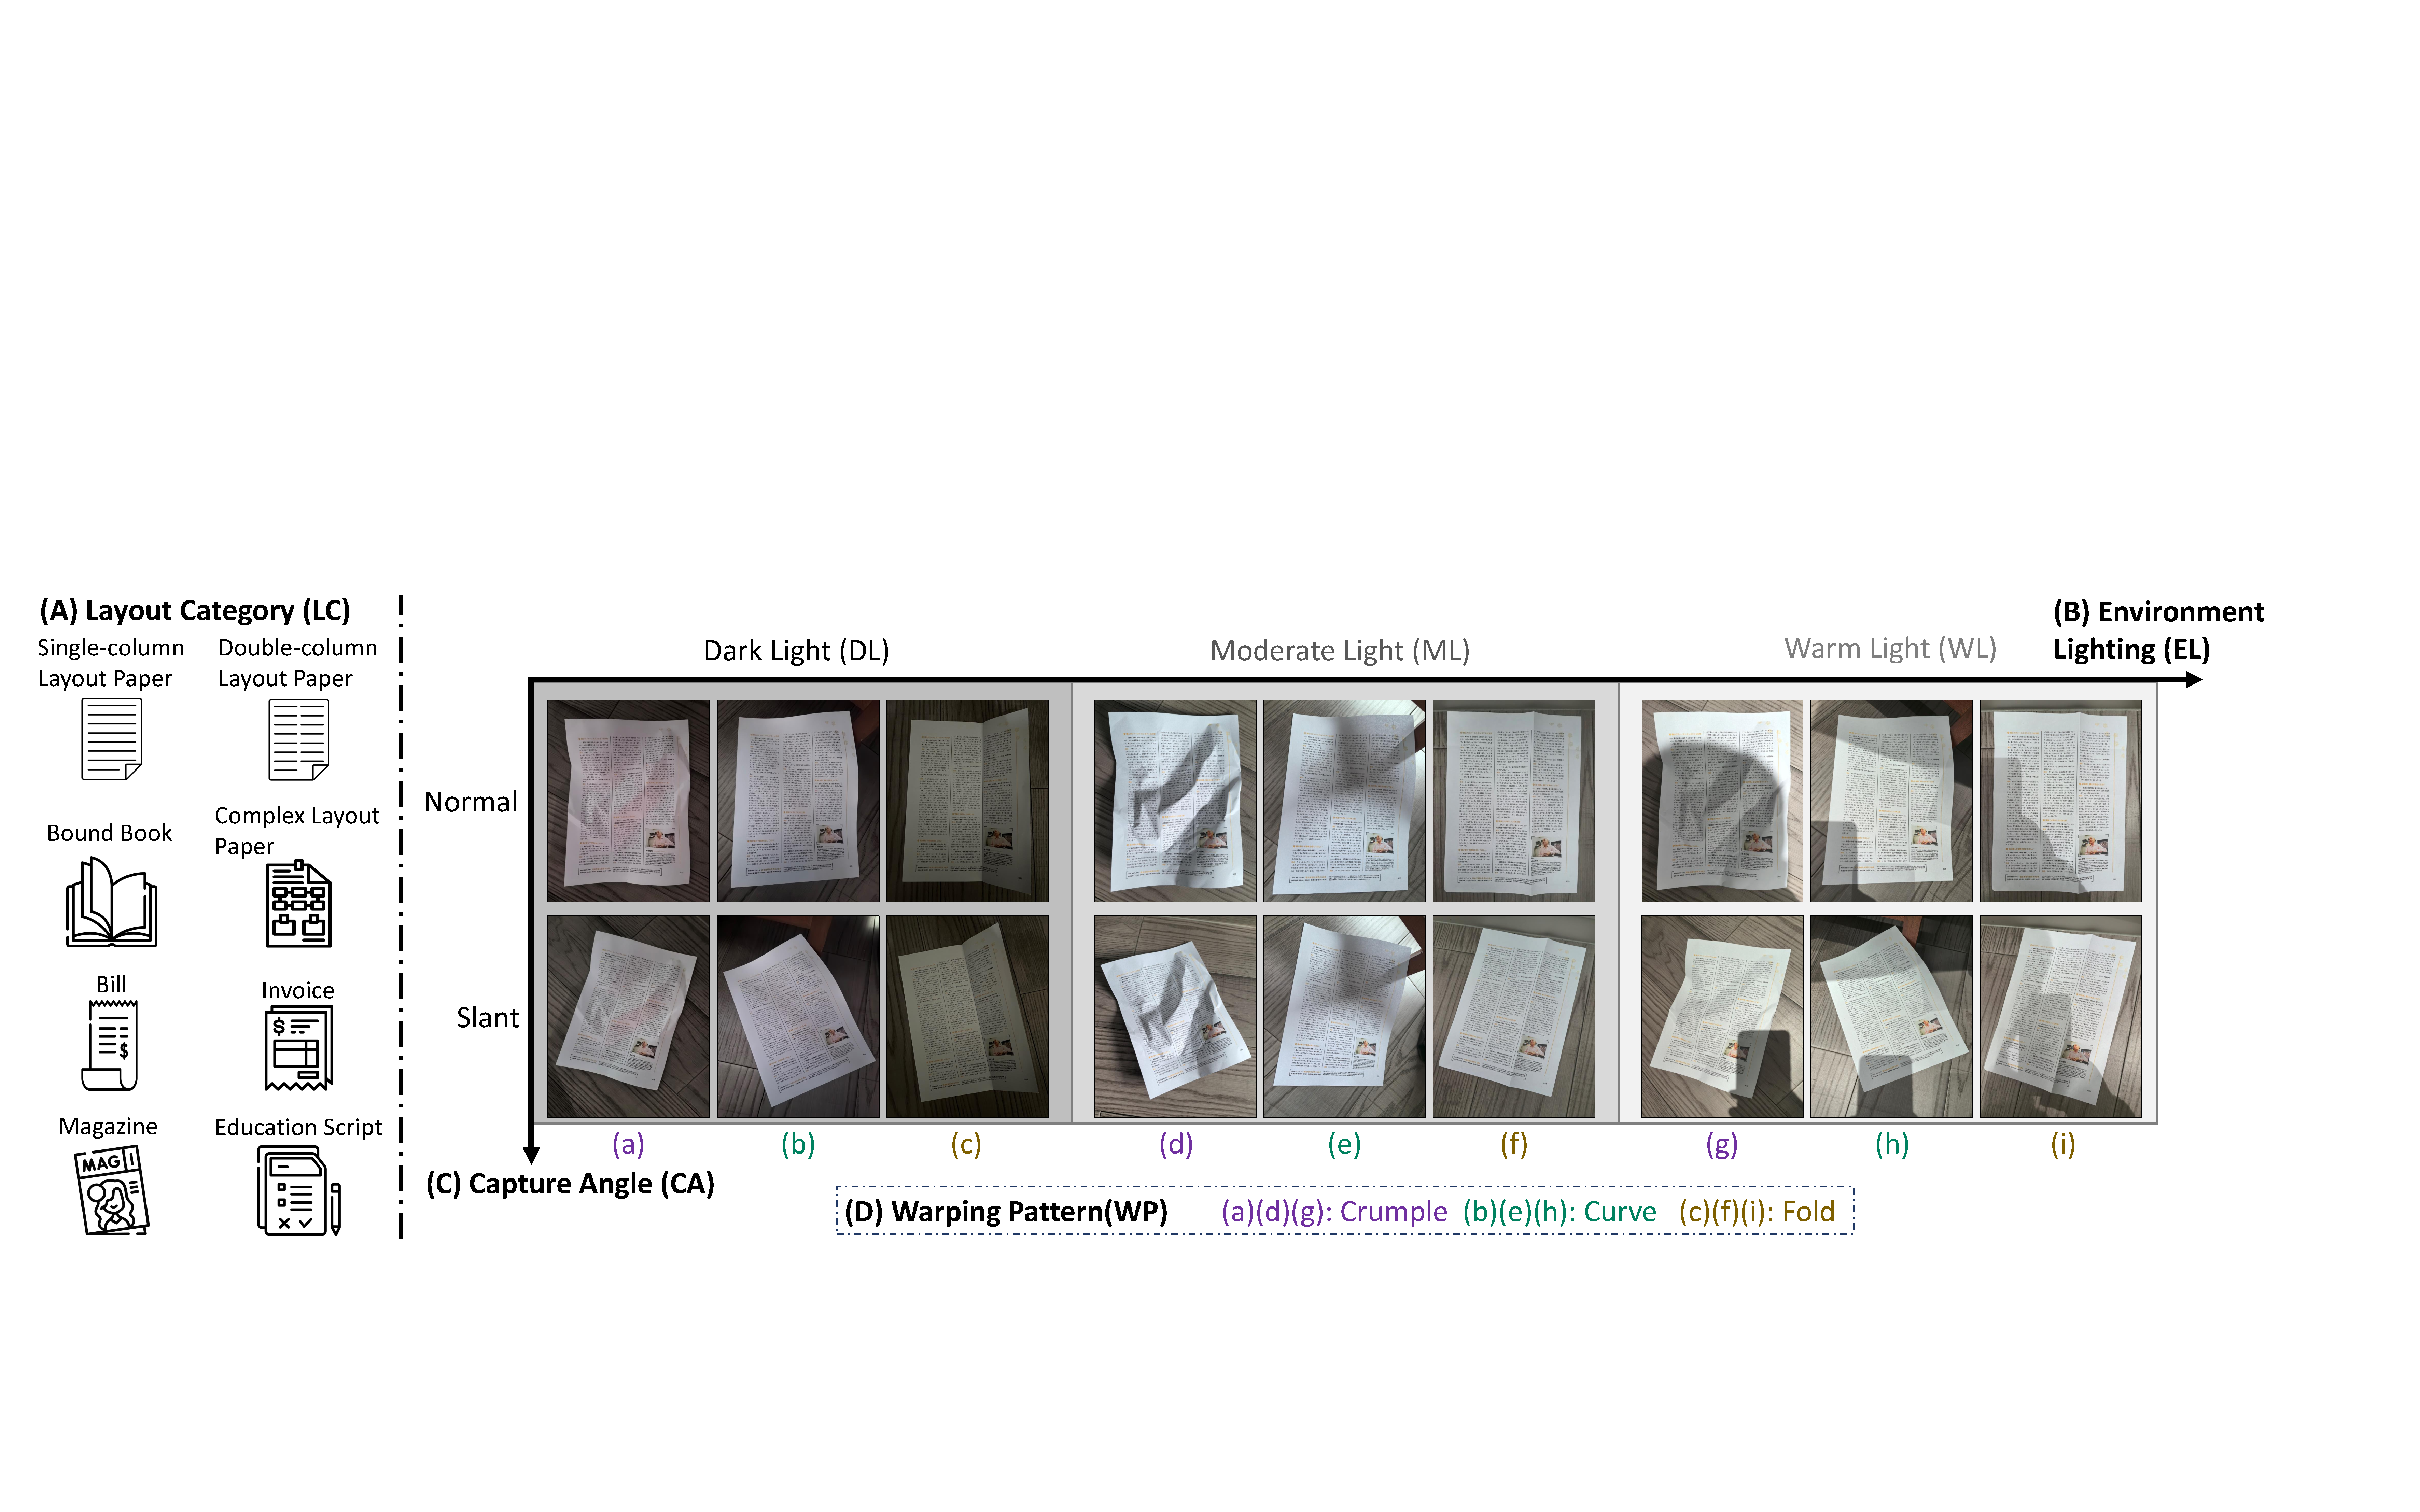
\includegraphics[width=0.98\linewidth]{figures/benchmark_v5.pdf}
	\caption{A sample data array visualization across 3 distinct domain spectra (A, B, C) in our AnyPhotoDoc6300 Benchmark. We aim to evaluate the dewarping capability of the model to different warping patterns (D) under well-distinguished domain combinations.}
\label{fig:benchmark_vis}
\end{figure*}



\subsection{Network Architecture}
\label{sec:method32}
In this section, we discuss the design of the network architecture in Fig.~\ref{fig:img2}, including the multiple feature extractors (\textbf{MFE}) and diffusion decoder. In MFE, we employ three parallel networks to extract features $f_d, f_m, f_l$ for raw document image, document foreground, and text lines, respectively. For document image features $f_d$, we utilize the first three blocks of VGG16~\cite{simonyan2014very} to extract features. For document foreground features $f_m$, we concatenate the last six layers of U2Net~\cite{qin_u2net_2020} as a foreground segmentation network to extract those features associated with foreground. For text lines features $f_l$, we use the last decoder layer of the UNet~\cite{ronneberger_unet_2015}, which is pre-trained for text-line segmentation. All extracted features are uniformly downsampled to $64\times64$ resolution compatible with the coordinate space.
Furthermore, as shown in Fig.~\ref{fig:network}, the diffusion decoder comprises 12 condition embedding blocks (\textbf{CEB}) and 6 fusion generation blocks (\textbf{FGB}). In each CEB, we extend the standard architecture of diffusion transformers (DiT), i.e.~DiT\_S\_2~\cite{Peebles_2023_dit} to implement both time embeddings and cross-attention conditioning.
To embed input time-steps, we adopt the same two-layer MLP in standard DiT to represent a 256-dimensional frequency embedding. To enable the condition control, we extend a multi-head cross-attention mechanism, where the compound condition $c_t$ serves as the key and value, and the noisy latent variable $m_t$ is used as the query. Specifically, we employ four parallel CEBs to decouple different conditions, including three feature conditions($f_d, f_m, f_l$) from the MFE and one time-variant condition ($r_t$). 
Subsequently, the CEB produces the hidden representations for the four conditions: $x_d$, $x_m$, $x_l$, and $x_r$.
In the FGB, the results of CEB are concatenated and fed into the FGB, which contains self-attention and feed-forward layers. Subsequently, we apply three linear layers as a projector to obtain the denoised mapping $m_0$. Next, we directly upsample $m_0$  to obtain the high-resolution mapping $M_0$, which is used to produce the final flat document image $I_0$ via Equ.~\ref{eq:def}. In Appendix B, we provide more detailed architectures.


% \qquad \FOR{each angle $\theta_b \in A $}
% \STATE  Emit a ray $r_b$ from $(x_0, y_0)$ with the $\theta_b$ direction
% \STATE  Find the intersection point $(x_b, y_b)$ of $r_b$ crossed $C_i$
% \STATE  \flushleft Calculate $ \rho'=\sqrt{(x_b-x_0)^2+(y_b-y_0)^2}$ as Euclidean radius 
% \STATE  Put $\rho'$ in $R_i$
% \ENDFOR
\begin{algorithm}[tp]
	\flushleft
	\caption{DvD training for TVCR mechanism}
	\begin{algorithmic}[1] %[1] enables line numbers
		\STATE  \textbf{repeat}
		\STATE  $m_0\sim q(m_0|c_t)$, $t \sim$ Uniform$(\{1,...,T\})$
		\IF{$t=T$} 
        \STATE  $r_T=\{O,O\}$, where $O$ represent all zeros for initialization 
        \ELSIF{$t<T$}
        \FOR{$t \in [T-1, t]$}
        \STATE  Sampling intermediate latent variable $m_{0|t}$ by Equ.~\ref{eq:reverse_ddim}
        \STATE  Using $m_{0|t}$ to obtain intermediate dewarped \\
                feature $f_{0|t}$ by Equ.~\ref{eq:def}
        \ENDFOR
        \STATE  $r_t=\{m_{0|t},f_{0|t}\}$
        \ENDIF
        \STATE $c_t=\{f_d,f_m,f_l,r_t\}$
		\STATE Optimize $m_{0|t}=\mathcal{\epsilon}_{\theta}(m_t, t, c_t)$ by Equ.~\ref{eq:loss}
		\STATE \textbf{until} Converged
	\end{algorithmic}
	\label{alg:training}
\end{algorithm}


\subsection{Training and Sampling}
\label{sec:method33}
\subsubsection{DvD Training Algorithm.}
Vanilla diffusion model randomly samples time-steps from a uniform distribution during the training phase~\cite{ho_2020_ddpm}, which mismatches the sequential acquisition of time-variant conditions. To solve this issue, we extend the vanilla diffusion model by integrating our TVCR mechanism, as detailed in Algorithm~\ref{alg:training}, where we implement a certain number of sampling based on current time-step, thereby obtaining the intermediate dewarping latent variables $m_{0|t}$ and the corresponding intermediate dewarped features $f_{0|t}$.





\subsubsection{Model Optimization.} During the training phase, we freeze the pre-trained weights of the foreground and text-line segmentation network from DocGeoNet~\cite{Feng2022geodocnet}, including U2Net and UNet. However, for the VGG dedicated to extracting raw document features, we jointly optimize it with the subsequent diffusion decoder. To optimize our DvD, instead of predicting noise in~\cite{ho_2020_ddpm}, we follow Luo et al.~\citeyearpar{luo2024flowdiffuser} and Nam et al.~\citeyearpar{nam_2024_diffmatch} to predict the generated object itself. Thus, the loss function is given by:
\begin{equation}
\begin{split}
\label{eq:loss}
\mathcal{L}=\mathbb{E}_{m_0\sim q(m_0|c_t), z \sim \mathcal{N}(\mathbf{0}, \mathbf{I}),t}\left[\left\|m_0-\mathcal{\epsilon}_\theta\left(m_t, t, c_t\right)\right\|^2\right],
\end{split}
\end{equation}


\subsubsection{Stochastic Sampling Property.} 
As shown in Equ.~\ref{eq:reverse_ddim}, the reverse process of DDIM~\cite{Alexander_2020_ddim} introduces $\sigma$ to inject stochasticity into the sampling trajectory. To account for this property and enhance generation stability, we implement a dual-hypothesis strategy that simultaneously generates two mappings. Afterward, we calculate the mean of the two mappings as a final result. We provide further training settings in Appendix A.


% We provide further training details available in supplementary materials A.
% Our DvD inherently inherits the diffusion model's capability to capture data probability distributions, thereby exhibiting potential to enhance its generalization to complex deformations in real-world scenarios. To validate this, we propose evaluating the generalization via real-world benchmarks. 

\begin{figure*}[htp]
	\centering
     % \setlength{\tabcolsep}{0.8pt}
     \renewcommand{\arraystretch}{1}
     \resizebox{\linewidth}{!}{
	\begin{tabular}{lccccccc}
\includegraphics[width=\linewidth]{figures/vis_comparison1_n.pdf}
        \\[-5pt]
        \scriptsize \hspace{3.7em}  (Input)
        \hspace{5.4em} \cite{das2019dewarpnet}
        \hspace{3.5em} \cite{RN58} 
        \hspace{3.6em} \cite{Feng2022geodocnet} 
        \hspace{2.1em} \cite{verhoeven2023neural} 
        \hspace{2.1em} \cite{li2023foreground} 
        \hspace{3.5em} (March,25th,2025)
        \hspace{5.3em} (Our)
        \\
	\end{tabular}}
	\caption{Qualitative comparisons on the AnyPhotoDoc6300 benchmark. We highlight some obvious content edges with red dotted lines. More visual comparisons can be found on the Figures-only pages after the reference.\label{fig:vis_compa1}}
\end{figure*}


\begin{table*}[htp]
\centering
\caption{Quantitative dewarping performance comparisons on the \hbox{DocUNet} benchmark dataset. \textbf{Bold} indicates the best, \underline{underline} indicates second-best. The last column shows the network size by the number of parameters (millions).}
\resizebox{\linewidth}{!}{%
	\begin{tabular}{r c c c c c c c c c c c c}
		\toprule
		Method &Venue &Training Dataset &MS-SSIM $\uparrow$ & LD $\downarrow$ & AD $\downarrow$ &  CER $\downarrow$ & ED $\downarrow$ &  MMCER $\downarrow$ & MMED $\downarrow$ & Para. \\
		\midrule
        Warped Document &- &- &0.246 & 20.51 & 1.026 & 0.595 & 1819.16 &0.576 &700.96 & - \\ \midrule
        \multicolumn{11}{c}{\cellcolor{gray!20}\textbf{Training under Non-uniform or Proprietary Dataset}} \\
		DispFlow~\cite{xie2020dewarping} &DAS'20 &DIWF &0.431 & 7.64 &0.411 & 0.446 &  1322.94 &0.887 &1339.43 & 23.6M  \\ 
		DDCP~\cite{xie2021document} &ICDAR'21 &DDCP &0.474 & 8.92 & 0.459  & 0.458 & 1335.30  &0.655 &762.28 & 13.3M \\
		PaperEdge~\cite{RN58} &SIGGRAPH'22 &Doc3D+DIW &0.472 &8.01 &0.385 & 0.407 & 1038.55 &\cellcolor{orange!45}\best{0.198} &530.27 & 36.6M  \\ 
		UVDoc~\cite{verhoeven2023neural} &SIGGRAPHA'23 &Doc3D+UVDoc &\cellcolor{orange!20}\second{0.544} &\cellcolor{orange!20}\second{6.83} &0.315 & 0.384 & 1026.91  &0.402 &615.88 & 8M \\
        LADoc~\cite{li2023ladoc} &TOG'23 &Doc3D+SP &0.523 &7.24 & 0.310 &0.395 &\cellcolor{orange!20}\second{956.27}  &0.242 &518.74 & -  \\
	DocReal~\cite{yu_docreal_2024} &WACV'24 &Doc3D+AugDoc3D &0.502 &7.00        &\cellcolor{orange!20}\second{0.284} &0.394 &1032.17 &0.336 &547.05 & -  
    \\ \midrule 	
        \multicolumn{11}{c}{\cellcolor{gray!20}\textbf{Training under Uniform Doc3D Dataset}} \\
		DewarpNet~\cite{das2019dewarpnet} &ICCV'19 &Doc3D &0.472 & 8.41 & 0.412 & 0.441 & 1158.66  &0.533 &734.84 & 86.9M\\ 
		DocTr~\cite{feng2021doctr} &MM'21 &Doc3D &0.511 & 7.77 &  0.365 & 0.403 & 1093.66 &0.432 &615.38  & 26.9M \\ 
		RDGR~\cite{jiang2022RDGR} &CVPR'22 &Doc3D&0.496 & 8.53 & 0.453 & 0.372 &994.01  &0.403 &534.97 & - \\
		Marior~\cite{jiaxin2022marior} &MM'22 &Doc3D &0.448  & 8.42 & 0.470 & 0.421 & 1131.48  &0.232 &\cellcolor{orange!45}\best{510.11} & - \\
		DocGeoNet~\cite{Feng2022geodocnet} &ECCV'22 &Doc3D &0.504  &7.69 & 0.378 & \cellcolor{orange!20}\second{0.367} & 993.08  &0.376 &627.11 & 24.8M \\ 
		FTA~\cite{li2023foreground} &ICCV'23 &Doc3D &0.494 &8.87 & 0.391 & 0.403 &1093.63  &0.355 &544.11 & 45.2M  \\
		DocScanner~\cite{feng2025docscanner} &IJCV'25 &Doc3D &0.523 &7.50 &0.333 &0.368 &1099.06  &- &- & 8.5M  \\        
		% \bottomrule 	
		DvD &- &Doc3D&\cellcolor{orange!45}\best{0.549} &\cellcolor{orange!45}\best{6.61} & \cellcolor{orange!45}\best{0.279} &\cellcolor{orange!45}\best{0.366} &\cellcolor{orange!45}\best{928.94}  &\cellcolor{orange!20}\second{0.215} &\cellcolor{orange!20}\second{515.97}
        & 151.25M \\\bottomrule
		% Ours w/o PP  & \best{7.24} & \best{0.382} & \best{0.246} & \best{868.88} & \best{9.6M} & \textbf{0.40}
\end{tabular}}
\label{tab:comparisontable}
\end{table*}



\section{Experiments}
\subsection{AnyPhotoDoc6300 Benchmark}
\label{sec:data}
Despite significant advances in document dewarping, the development of corresponding benchmarks lags behind. We summarized current benchmarks in Tab.~\ref{tab:unwarping_datasets}, and we can find most of datasets suffer from restricted coverage of scenarios, small size of dataset, and deficient annotations of domains, impeding a comprehensive evaluation of dewarping models. To this end, we build a new large-scale benchmark AnyPhotoDoc6300, containing 6,300 real-world photographic document pairs. In our AnyPhotoDoc6300, we provide three distinct domain annotations to enable a more fine-grained quantitative evaluation, including layout category (LC), environment lighting (EL), and capture angles (CA). 
%To overcome the limitations (i.e., restricted scenario coverage, small dataset scale, and deficient domain annotations) in current benchmarks and enable a more fine-grained quantitative evaluation, we construct AnyPhotoDoc6300, a large-scale benchmark containing 6,300 
%real-world photographic document pairs with three distinct domain annotations, including layout category (LC), environment lighting (EL), and capture angles (CA). 
In addition, we aim to evaluate the dewarping capability of the model on three typical warping patterns (i.e., curves, folds, and crumples) under any combination of three types of given domains.
Fig.~\ref{fig:benchmark_vis} visualizes a sample array of "Complex layout paper" (one of the eight layout categories). 
By meticulously specifying three environmental lighting and two capture angles, we can form any domain combination for the same document content. Consequently, we can obtain a fine-grained performance evaluation like Fig.~\ref{fig:vis_comparison0} to discover the underlying issues for the current dewarping model. In Appendix E, we provide more details about our AnyPhotoDoc6300 benchmark, including data collection settings and more visualizations from different layout categories. 
% We put some examples of AnyPhotoDoc6300 benchmark in Appendix E.  


% (1) We first fix one texture from the 8 LP (i.e.,~the complex layout paper in Fig.~\ref{fig:benchmark_vis} (A)), and then (2) control the different domains through 3 EL and 2 CA. 
% Under any combination of these 3 disentangled domain parameters, we systematically capture documents with 3 types of warping patterns (Crumple, curve, and fold) for different deformations evaluation. 
% Through this meticulous configuration, AnyPhotoDoc6300 enables fair evaluation of model generalization across subdivided warping patterns while maintaining domain variable isolation. 






\subsection{Metrics}
\label{sec:metric}
\subsubsection{Feature Alignment Metrics.} Following most of previous models~\cite{ma2018docunet, das2019dewarpnet, RN58}, we adopt the MS-SSIM (Multi-scale Structural Similarity)~\cite{msssim2003}, LD (Local Distortion)~\cite{ld2017}, and AD (Aligned Distortion)~\cite{RN58} to evaluate differences between dewarped and flat ground truth. Among them, MS-SSIM focuses on perceiving similarity on luminance, contrast, and structural information. While LD and AD focus on measuring the variations of SIFT flow~\cite{liu2010sift}.


%In addition, as shown in Tab. 1, we find that existing publicly
% available document dewarping benchmarks suffer from three critical
% limitations that impede a comprehensive evaluation of dewarping
% models, including narrow scenario coverage, restricted dataset scale,
% and deficient domain annotations. These limitations might have
% led to evaluation ambiguity, restricting the model’s application in
% real-world scenarios. To this end, we construct a fine-grained and
% large-scale benchmark, dubbed AnyPhotoDoc6300, which contains
% 6,300 real-world photographic image document pairs, rigorously
% organized across three distinct domains, enabling fine-grained eval-
% uation of dewarping models.

% However, as shown in Tab.~\ref{tab:unwarping_datasets}, none of the existing benchmarks enable fair evaluation of generalization. 
% Particularly, DocReal~\cite{yu_docreal_2024} and Inv3DReal~\cite{hertlein2023inv3d} focus on specific scenarios (i.e., invoices and Chinese documents).
% UVDoc~\cite{verhoeven2023neural} adopts synthetic documents to moderate domain entanglement caused by environmental lighting variations.
% DocUNet~\cite{ma2018docunet} and DIR300~\cite{Feng2022geodocnet} coarsely mix hundreds of documents from multiple scenarios without distinguishing domains explicitly, constituting inherent domain entanglement.
% Although DocUNet and DIR300 remain the most widely used benchmarks for document dewarping, their severe domain entanglement introduces evaluation ambiguity, fundamentally limiting their utility for more elaborate analysis (e.g., generalization assessment). 
% We provide a visual example in Appendix B to demonstrate this issue.

% To address these deficiencies, we construct AnyPhotoDoc6300, a well-organized benchmark containing 6,300 real captured document pairs across 3 distinct domains, including layout patterns (LP), environment lighting (EL), and capture angles (CA). Fig.~\ref{fig:benchmark_vis} visualizes a sample array from our AnyPhotoDoc6300. (1) We first fix one texture from the 8 LP (i.e.,~the complex layout paper in Fig.~\ref{fig:benchmark_vis} (A)), and then (2) control the different domains through 3 EL and 2 CA. 
% Under any combination of these 3 disentangled domain parameters, we systematically capture documents with 3 types of warping patterns (Crumple, curve, and fold) for different deformations evaluation. 
% Through this meticulous configuration, AnyPhotoDoc6300 enables fair evaluation of model generalization across subdivided warping patterns while maintaining domain variable isolation. More details of the benchmark set can be found in Appendix D.





\begin{figure*}[htp]
	\centering
	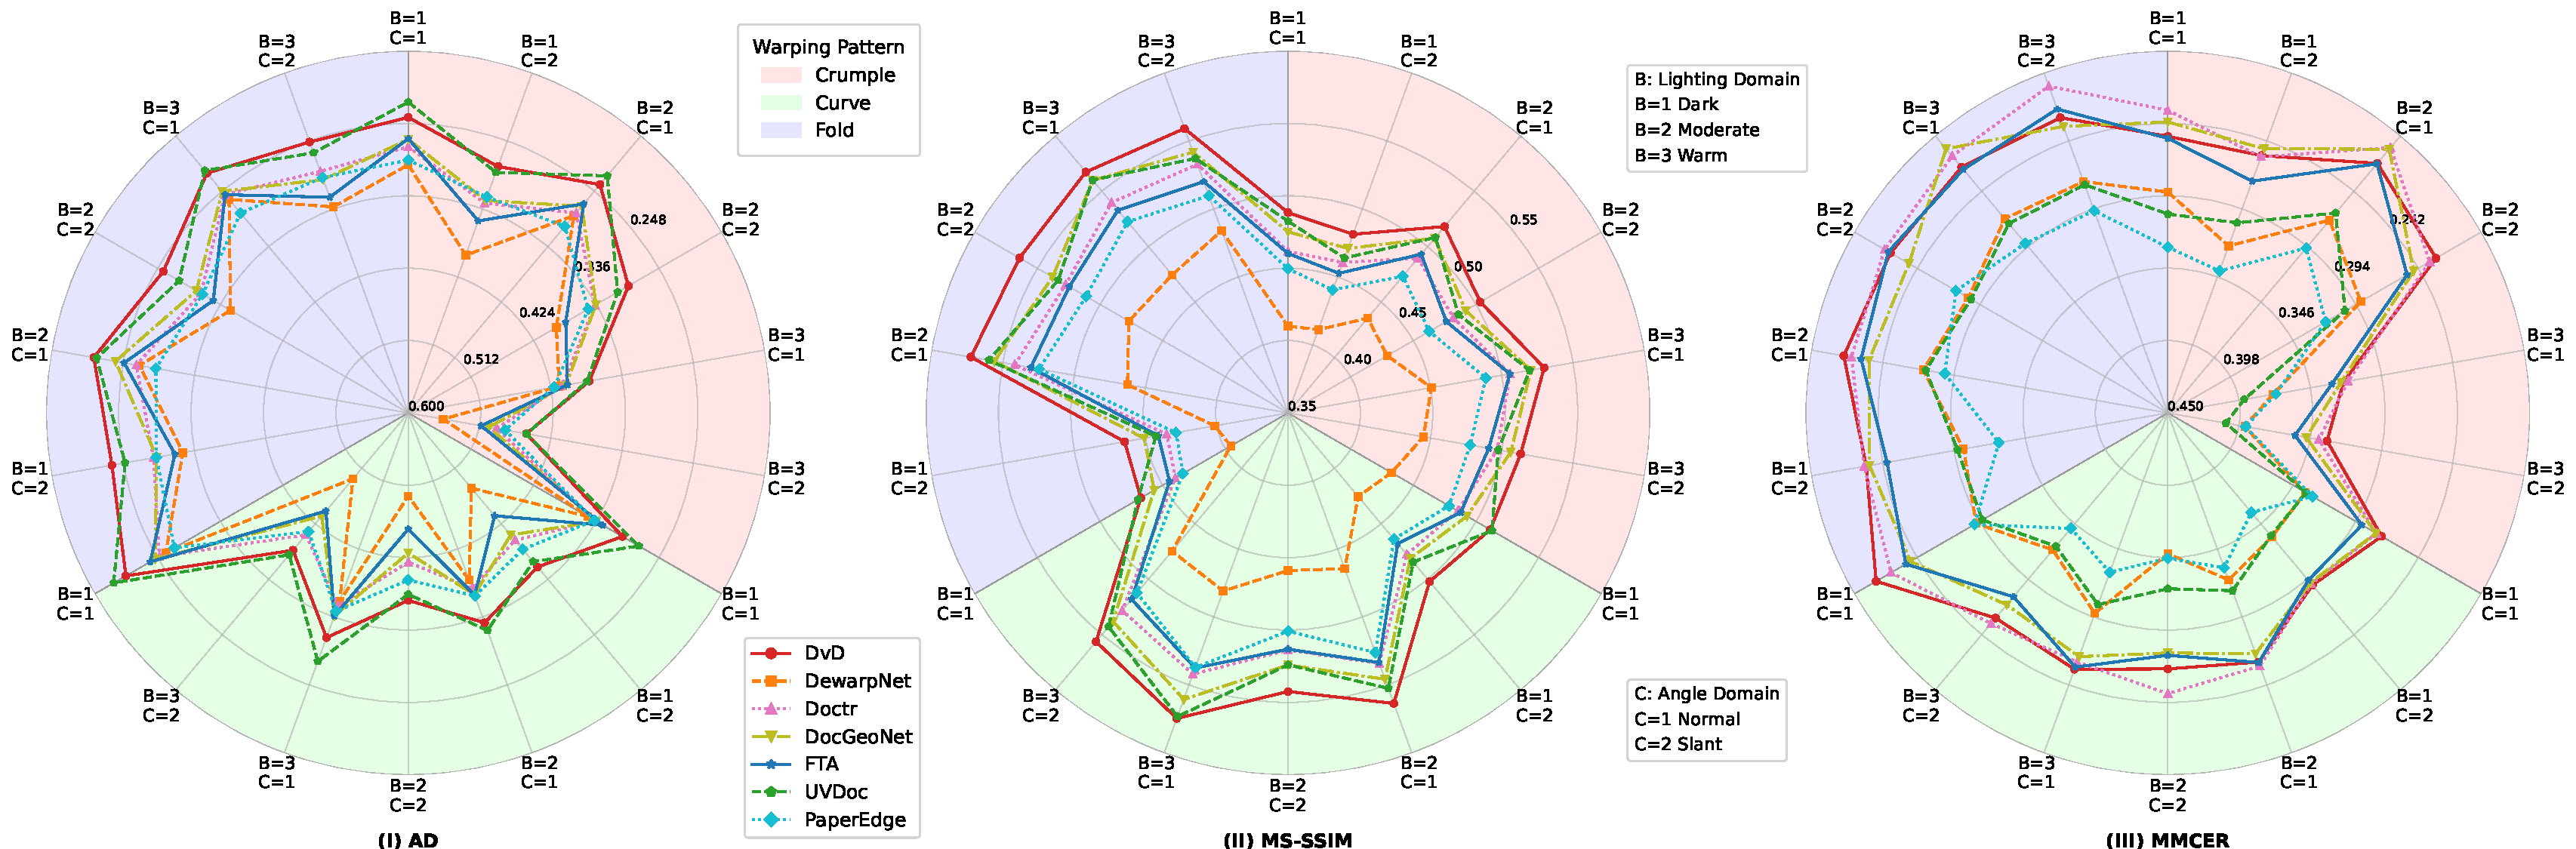
\includegraphics[width=\linewidth]{figures/combined_radars_ftotal.pdf}
	\caption{Quantitative dewarping performance comparisons on the \hbox{AnyPhotoDoc6600} benchmark dataset. Under the multiple Layout Pattern, we provided 18 dimensions of evaluation for AD, MS-SSIM, and MMCER. More evaluation results can be found on the Figures-only pages after the reference.}
\label{fig:vis_comparison0}
\end{figure*}










\subsubsection{OCR Metrics.} 
To evaluate the OCR readability improvement enabled by document dewarping, measuring recognition discrepancy between dewarped and flat documents has become the de facto standard in contemporary document dewarping models. Concretely, an off-the-shelf OCR engine is applied to recognize two text sequences from dewarped and flat documents, respectively. Then, ED (Edit Distance) and CER (Character Error Rate) ~\cite{levenshtein1966binary} are harnessed to quantify the degree of deviation between two sequences. 
Pioneering a metric supplement, we further extend current OCR metrics in document dewarping by replacing previous OCR engines with MLLMs.
Witnessing the superior progress of MLLMs in OCR capabilities recently~\cite{wei2024general, karmanov_eclair_2025, nassar_smoldocling_2025}, we identify that there is still no exploration about whether the dewarped document can attain equivalent readability to its flat counterpart for MLLMs.
To fill the blank, we pioneer MLLM-based OCR metrics (i.e., MMCER, MMED) to serve as a specialized supplement for prevalent ED and CER.
Specifically, given the prompt of "OCR the plain text" as a fixed instruction, we employ open-source MLLM QWen2.5-VL 7B~\cite{bai_2025_qwen25vl} to recognize all characters in both dewarped and flat documents for ED and CER calculation.




% As there are no ground-truth string annotations, current dewarping models commonly adopt an OCR engine to recognize the ground-truth document image to obtain the reference string.

% Additionally, existing methods commonly utilize off-the-shelf OCR engines to measure the Edit Distance (ED) and Character Error Rate (CER) as OCR metrics~\cite {das2019dewarpnet}. 
% % We identify that there is no exploration about whether document dewarping is still useful for OCR using MLLMs. 
% We identify that there is still no exploration about the extent to which dewarped documents can enhance text readability in MLLMs. 
% To fill the blank, we contribute MLLM-based OCR metrics (i.e.,~MMCER, MMED) to serve as a specialized supplement for prevalent ED and CER. 

\subsection{Qualitative and Quantitative Comparison}
\subsubsection{Qualitative Comparisons.} Dewarped document results on the AnyPhotoDoc6300 and DocUNet benchmark are shown in Fig.~\ref{fig:vis_compa1}. 
In this figure, we select the five most recent open‑source dewarping models as well as GPT‑4o’s native generation model. Our prompt fed to GPT-4o is consistently given, i.e., "Please perform dewarping on this document to make it flat and clear.". On Fig.~\ref{fig:vis_compa2} and Fig.~\ref{fig:vis_compa3}, we additionally compare against publicly released inference results from non‑open‑source methods. Basically, our DvD achieves precise structure preservation in both local and overall document content. In contrast, GPT‑4o tends to produce unfaithful results that look visually clean but whose content is often chaotic. We argue this is because the image translation paradigm adopted by GPT-4o lacks explicit deformation awareness.

\subsubsection{Quantitative Comparisons.}
We compare the performance of our DvD model with previous state-of-the-art on three benchmarks, including DocUNet~\cite{ma2018docunet}, DIR300~\cite{Feng2022geodocnet}, and the proposed AnyPhotoDoc6300. 
The quantitative results on the DocUNet benchmark are shown in Tab.~\ref{tab:comparisontable}. For DIR300, we have placed the results in Appendix C. The "Warped Document" in the first row means that we simply feed the raw input image for evaluation, therefore, most of the metrics perform the worst.
Since our paper focuses on novel model designs rather than contributing high-quality data, we only train DvD on the currently most widely used Doc3D~\cite{das2019dewarpnet} dataset. For a fair comparison, we divide the current methods into two branches according to their training data. It can be seen that even though we only used the Doc3D dataset, our method still achieved the best performance on the majority of metrics.
In the upper first branch, DvD can achieve a slight overtaking, while in the lower second branch, DvD can achieve a significant superiority under a uniform Doc3D dataset. To be noted, compared with the first row, our experiments on MMCER and MMED reveal counterintuitive performance degradation in earlier dewarping models (e.g., DispFlow, DewarpNet), which we attribute to the fact that MLLMs are sensitive to resolution reduction and artifact~\cite{Li_2024_CVPR, feng_docpedia_2024}. On the other hand, compared with the first row, our DvD significantly reduces MMCER and MMED, and greatly improves the perception of photographed documents for MLLMs.


\subsubsection{Fine-grained Quantitative Comparisons.}
Fig.~\ref{fig:vis_comparison0} illustrates AD, MS‑SSIM, and MMCER as three representative metrics via the Any-PhotoDoc6300 benchmark. More metrics in different domains are also exhibited in the Fig.~\ref{fig:vis_comparison},\ref{fig:vis_comparison2},\ref{fig:vis_comparison3}, and Appendix. Our DvD comprehensively achieves superior performance across various domains, including layout, lighting, and angles. Moreover, for the first time, we can also unveil some brand-new performance comparisons for dewarping models at a fine-grained level. For instance, in Fig.~\ref{fig:vis_comparison0} (I), existing methods generally suffer from severe AD performance decline under mixed warm lighting and slant angle, especially on the warping pattern of the curves and crumple.
In Fig.~\ref{fig:vis_comparison0} (II), we observe a notable MS-SSIM drop for dark lighting documents.
In Fig.~\ref{fig:vis_comparison0} (III), warm lighting causes the most pronounced decline in OCR metrics, especially on crumpled documents.
By pinpointing these issues unconventionally, we expect to provide the research community deeper insights into dewarping model behaviors and dataset curation, for driving further performance improvements.




\subsection{Ablation Studies}
% In this section, we conduct the ablation studies on the DocUNet benchmark from three aspects, including the (1) Effectiveness of the "Noise-to-Flow" generative paradigm in DvD, (2) Component analysis of compound conditions, and (3) Computational efficiency analysis. The first two are respectively presented in Tab.~\ref{tab:ablation1} and Tab.~\ref{tab:ablation2}, while the experiment on the third aspect is further analyzed in Appendix E.
\subsubsection{Effectiveness on different Dewarping Paradigms.}
To verify the superiority of the proposed paradigm over the regression-based paradigm, we specially train another network of DvD by directly regressing the mapping. Then we can fairly compare different learning paradigms under the same network structure. As demonstrated in Tab.~\ref{tab:ablation1}, The DvD baseline model trained using the regression-based paradigm has led to a general decline in performance, which emphasizes the effectiveness of our mapping generation paradigm for obtaining a more precise structure preservation.

\subsubsection{Component Analysis of Compound Conditions.}
Tab.~\ref{tab:ablation2} demonstrates three types of compound condition $c_t$ configurations. We can see that only using the raw document feature $f_d$ does not obtain satisfactory performance, which is then improved by adding the document foreground $f_m$ and text-lines $f_l$. Finally, adding a time-variant condition $r_t$ further boosts the performance, obviously on all metrics. All of these verify the complementarity of those compound conditions.  
%When we only use the raw document feature $f_d$ or add document foreground $f_m$ and text-lines $f_l$, the best performance cannot be achieved. The time-variant condition $r_t$ corresponds to the TVCR mechanism we proposed in Sect.~\ref{sec:method31}. 
%When we select the combination of four conditions, we obtain the optimal performance, which verifies the effectiveness of each condition along with the TVCR mechanism.

\begin{table}[tp]
\centering\caption{Ablation study on different learning paradigms.}
\vspace{-5pt}
\resizebox{\linewidth}{!}{
   \begin{tabular}{lccccc}
        \toprule
         Learning paradigms &MS-SSIM $\uparrow$ & LD $\downarrow$ & AD $\downarrow$ &  CER $\downarrow$ & ED $\downarrow$
         \\
        \midrule
DvD (Mapping Regression)  & 0.487 &7.85 &0.482 &0.410 &1084.67 \\
DvD (Mapping Generation) &\textbf{0.549} &\textbf{6.61} &\textbf{0.279} &\textbf{0.366} &\textbf{928.94} \\
        \bottomrule
\end{tabular}}
\label{tab:ablation1}
\end{table}



\begin{table}[tp]
\centering\caption{Ablation study for different conditions components}
\vspace{-5pt}
\resizebox{0.88\linewidth}{!}{
\begin{tabular}{ccc|ccccc}
\toprule
\multicolumn{3}{c|}{Conditions $c_t$} & \multicolumn{5}{c}{ Experimental Results } \\ 
 $f_d$ & $f_m,f_l$  & $r_t$    &MS-SSIM $\uparrow$ & LD$\downarrow$ & AD $\downarrow$ & CER $\downarrow$ & ED $\downarrow$\\
\midrule
$\checkmark$ & &               &0.409  & 8.18 &0.332 & 0.427 & 1184.52\\
$\checkmark$ &$\checkmark$ &   &0.519 & 7.12 & 0.323 & 0.408 & 1046.71\\
$\checkmark$ &$\checkmark$ &$\checkmark$ &\textbf{0.549} &\textbf{6.61} &\textbf{0.279} &\textbf{0.366} &\textbf{928.94}\\
\bottomrule
\hline
\end{tabular}}
\label{tab:ablation2}
\end{table}


\begin{table}[tp]
\caption{Ablations on sampling step, performance, and time consumption.}
\vspace{-5pt}
\centering
\resizebox{0.92\linewidth}{!}{
\color{black}{
   \begin{tabular}{l|cccccc}
        \toprule
        Steps &MS-SSIM $\uparrow$ & LD$\downarrow$ & AD $\downarrow$ & CER $\downarrow$ & ED $\downarrow$ & Time $\downarrow$ \\ \midrule
        1  &0.420 &9.86 &0.501 &0.875 &1952.54 &\textbf{0.21}\\ 
        3   &\textbf{0.549} &\textbf{6.61} &\textbf{0.279} &\textbf{0.366} &\textbf{928.94} & 0.59\\ 
        5   &0.537 &6.60 &0.281 &0.372 &956.46 &1.06\\
        50  &0.475 &7.56 &0.467 &0.441 &1261.43 &10.32\\
        \bottomrule
\end{tabular}}}
\label{tab:ablation3} 
\end{table}

\begin{table}[tp]
\caption{Ablations study for different latent size.}
\vspace{-5pt}
\centering
\resizebox{0.82\linewidth}{!}{
\color{black}{
   \begin{tabular}{c|ccccc}
        \toprule
        Size &MS-SSIM $\uparrow$ & LD$\downarrow$ & AD $\downarrow$ & CER $\downarrow$ & ED $\downarrow$  \\ \midrule
        $16\times16$  &0.432 &10.63 &0.462 &0.451 &1343.87 \\ 
        $32\times32$   &0.492 &7.69 &0.370 &0.385 &1023.28 \\ 
        $64\times64$  &0.549 &\textbf{6.61} &0.279 &\textbf{0.366} &\textbf{928.94} \\
        $128\times128$  &\textbf{0.551}&6.62&\textbf{0.276}&0.376&940.43\\
        \bottomrule
\end{tabular}}}
\label{tab:ablation4} 
\end{table}

\subsubsection{Computational Efficiency Analysis.}
Tab.~\ref{tab:ablation3} illustrates a trade-off between performance and time consumption, driven by different diffusion denoising steps. The time unit here refers to the average elapsed seconds per image we take to infer the DocUNet~\cite{ma2018docunet} benchmark. As the number of sampling steps increases from 1 to 3, the model’s performance improves substantially. However, beyond 3 steps, performance largely plateaus or even slightly declines. We consider that this might be due to excessive steps that could accumulate errors over time, causing generated samples to deviate from the real distribution. At the same time, increasing the step count incurs a linearly growing time cost. In our experiments, we set 3 as the optimal step setting for a trade-off between performance and time consumption.

\subsubsection{Size Analysis for Latent Space.}
Tab.~\ref{tab:ablation4} presents the performance of the DvD model under different latent space resolutions. When the resolution is too small ($16\times16$), the model performs poorly. We attribute this to the fact that such a limited latent space sacrifices overmuch warping semantics, making it difficult to accurately represent the high-resolution (i.e., $2000\times3000$) backward mapping $M_0$. Empirically, we find that a moderate resolution of $64\times64$ is sufficient to provide warping semantics. Further increasing the resolution to $128\times128$ yields no significant performance gain.





% (3) Second-best LD metric: Although DvD outperforms overall on AnyPhotoDoc6300, it achieves only the second-best result on the LD metric (See Table7 in the Appendix). We speculate that this may be due to the model’s insufficient ability to learn deformation from texture-less regions.



\subsubsection{Limitations.} 
Our method still has two limitations. (1) Slow training: Unlike directly selecting the denoising time-step in vanilla DDIM, training with the TVCR mechanism requires sampling a few steps per iteration, causing a slower training speed.
(2) Limited Generalization on unseen document types: Diffusion models excel at generating samples that conform to the training data distribution. Since the training set Doc3D~\cite{das2019dewarpnet} contains many academic papers and magazines, DvD shows superiority on these seen document types (cf. Fig.~\ref{fig:vis_comparison},\ref{fig:vis_comparison2},\ref{fig:vis_comparison3}). However, DvD's improvements on unseen types (Invoices/Education scripts) are negligible (cf. Fig.~15,16 in Appendix).
% (3) Second-best LD metric: Although DvD outperforms overall on AnyPhotoDoc6300, it achieves only the second-best result on the LD metric (See Table7 in the Appendix). We speculate that this may be due to the model’s insufficient ability to learn deformation from texture-less regions.
% Fig.~\ref{fig:vis_comparison5},\ref{fig:vis_comparison6}




% \item We present DvD, the first generative model to tackle document \textbf{D}ewarping \textbf{v}ia a conditional \textbf{D}iffusion framework, moving beyond the previous regression-based paradigm. 
% \item To improve structural preservation, we operate denoising in coordinate space instead of pixel space to explicitly foster deformation-aware modeling. Meanwhile, we introduce a time-variant condition refinement mechanism to leverage intermediate dewarping results as dynamic guidance.
% \item To evaluate generalization inherited from diffusion model, we construct AnyPhotoDoc6300, an organized, large-scale benchmark across 3 distinct domains. Additionally, we propose MLLM-based OCR metrics to supplement prevalent ED and CER. It pioneers an exploration of whether dewarping is still useful for MLLMs.


\section{Conclusion}
% moving beyond the previous mapping regression paradigm. 
This paper unleashes a novel mapping generation paradigm for the document dewarping task by reformulating it as a coordinate-based denoising diffusion framework.
To the best of our knowledge, this is the first attempt to explore the viability of dewarping a document using the diffusion model, where we tailor a coordinate‑level denoising strategy and a time-variant condition refinement (TVCR) mechanism, enabling precise preservation of document structures.
To foster a fine-grained evaluation of dewarping models, we also build a new photographic document dewarping benchmark, AnyPhotoDoc 6300, which is large-scale in size, covers multiple scenarios, and provides detailed domain annotations.
Findings and insights from our experiments are poised to substantially advance photographic document processing and further impact a broad spectrum of graphics applications.

\begin{acks}
The work was partially supported by the following: National Natural Science Foundation of China under No. 92370119, 62436009, 62276258 and 62376113, XJTLU Funding REF-22-01-002.
\end{acks}

\begin{figure*}[htp]
	\centering
     % \setlength{\tabcolsep}{0.8pt}
     \renewcommand{\arraystretch}{1}
	\begin{tabular}{lccccccc}
\includegraphics[width=\linewidth]{figures/vis_comparison2_n.pdf}
        \\[-6.2pt]
        \scriptsize \hspace{3.9em}  (Input)
        \hspace{4.4em} \cite{jiaxin2022marior}
        \hspace{1.9em} \cite{verhoeven2023neural} 
        \hspace{2.2em} \cite{li2023ladoc} 
        \hspace{3.8em} \cite{li2023foreground} 
        \hspace{3.9em} \cite{yu_docreal_2024} 
        \hspace{3.5em} (March,25th,2025)
        \hspace{5.3em} (Our)
        \\
	\end{tabular}
	\caption{More Qualitative comparisons on the DocUNet benchmark. We highlight some obvious content edges with red dotted lines. \label{fig:vis_compa2}}
\end{figure*}


\begin{figure*}[htp]
	\centering
     % \setlength{\tabcolsep}{0.8pt}
     \renewcommand{\arraystretch}{1}
	\begin{tabular}{lccccccc}
\includegraphics[width=\linewidth]{figures/vis_comparison3_n.pdf}
        \\[-6.2pt]
        \scriptsize \hspace{3.6em}  (Input)
        \hspace{5.4em} \cite{das2019dewarpnet}
        \hspace{3.5em} \cite{RN58} 
        \hspace{3.7em} \cite{Feng2022geodocnet} 
        \hspace{1.9em} \cite{verhoeven2023neural} 
        \hspace{2.1em} \cite{li2023foreground} 
        \hspace{3.5em} (March,25th,2025)
        \hspace{5.3em} (Our)
        \\
	\end{tabular}
	\caption{More Qualitative comparisons on the AnyPhotoDoc6300 benchmark. We highlight some obvious content edges with red dotted lines. \label{fig:vis_compa3}}
\end{figure*}


\begin{figure*}[htp]
	\centering
	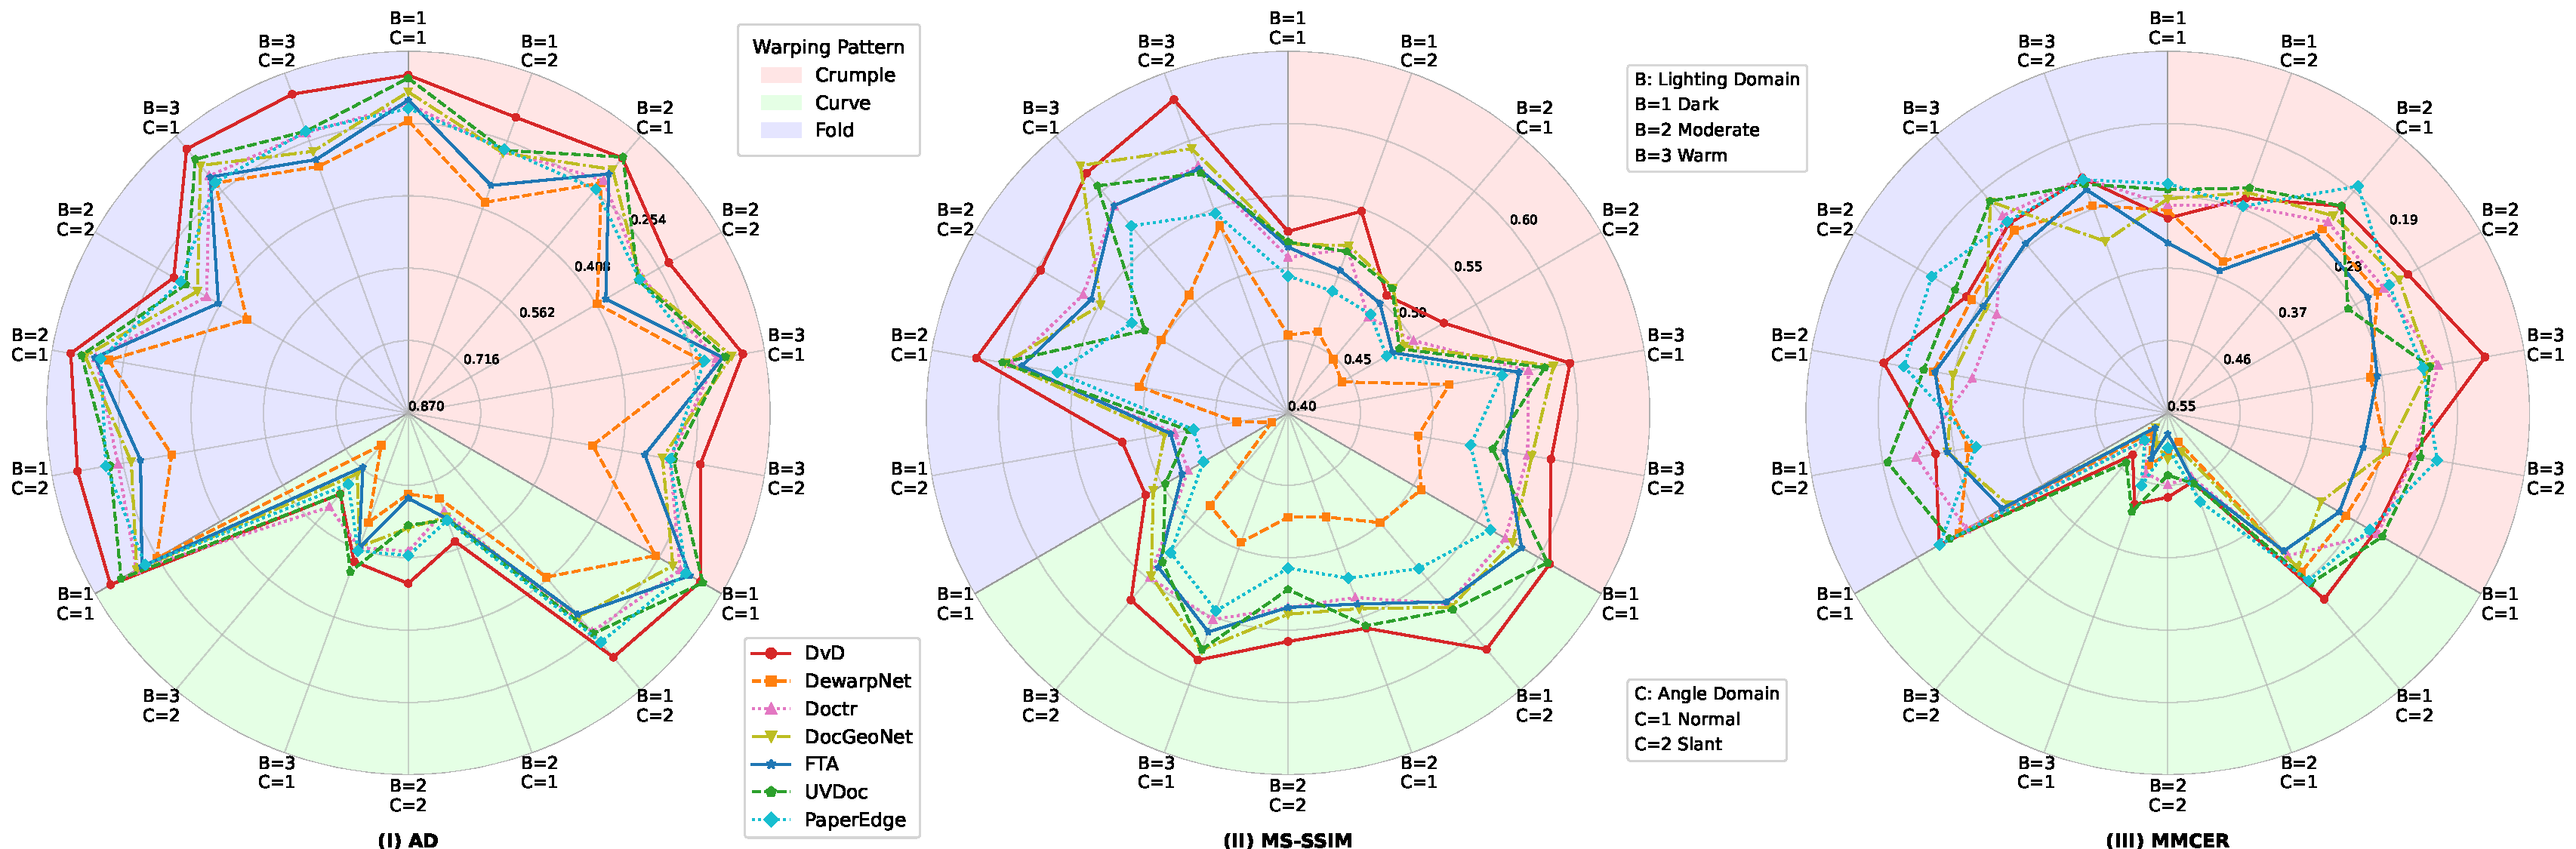
\includegraphics[width=\linewidth]{figures/combined_radars_f6.pdf}
	\caption{Quantitative dewarping performance comparisons on the \hbox{AnyPhotoDoc6600} benchmark dataset. Under the fixed "Two-column Paper" Layout Pattern, we provided 18 dimensions of evaluation for AD, MS-SSIM, and MMCER. More evaluation results can be found on the Figures-only pages after the reference.}
\label{fig:vis_comparison}
\end{figure*}

\begin{figure*}[tp]
	\centering
	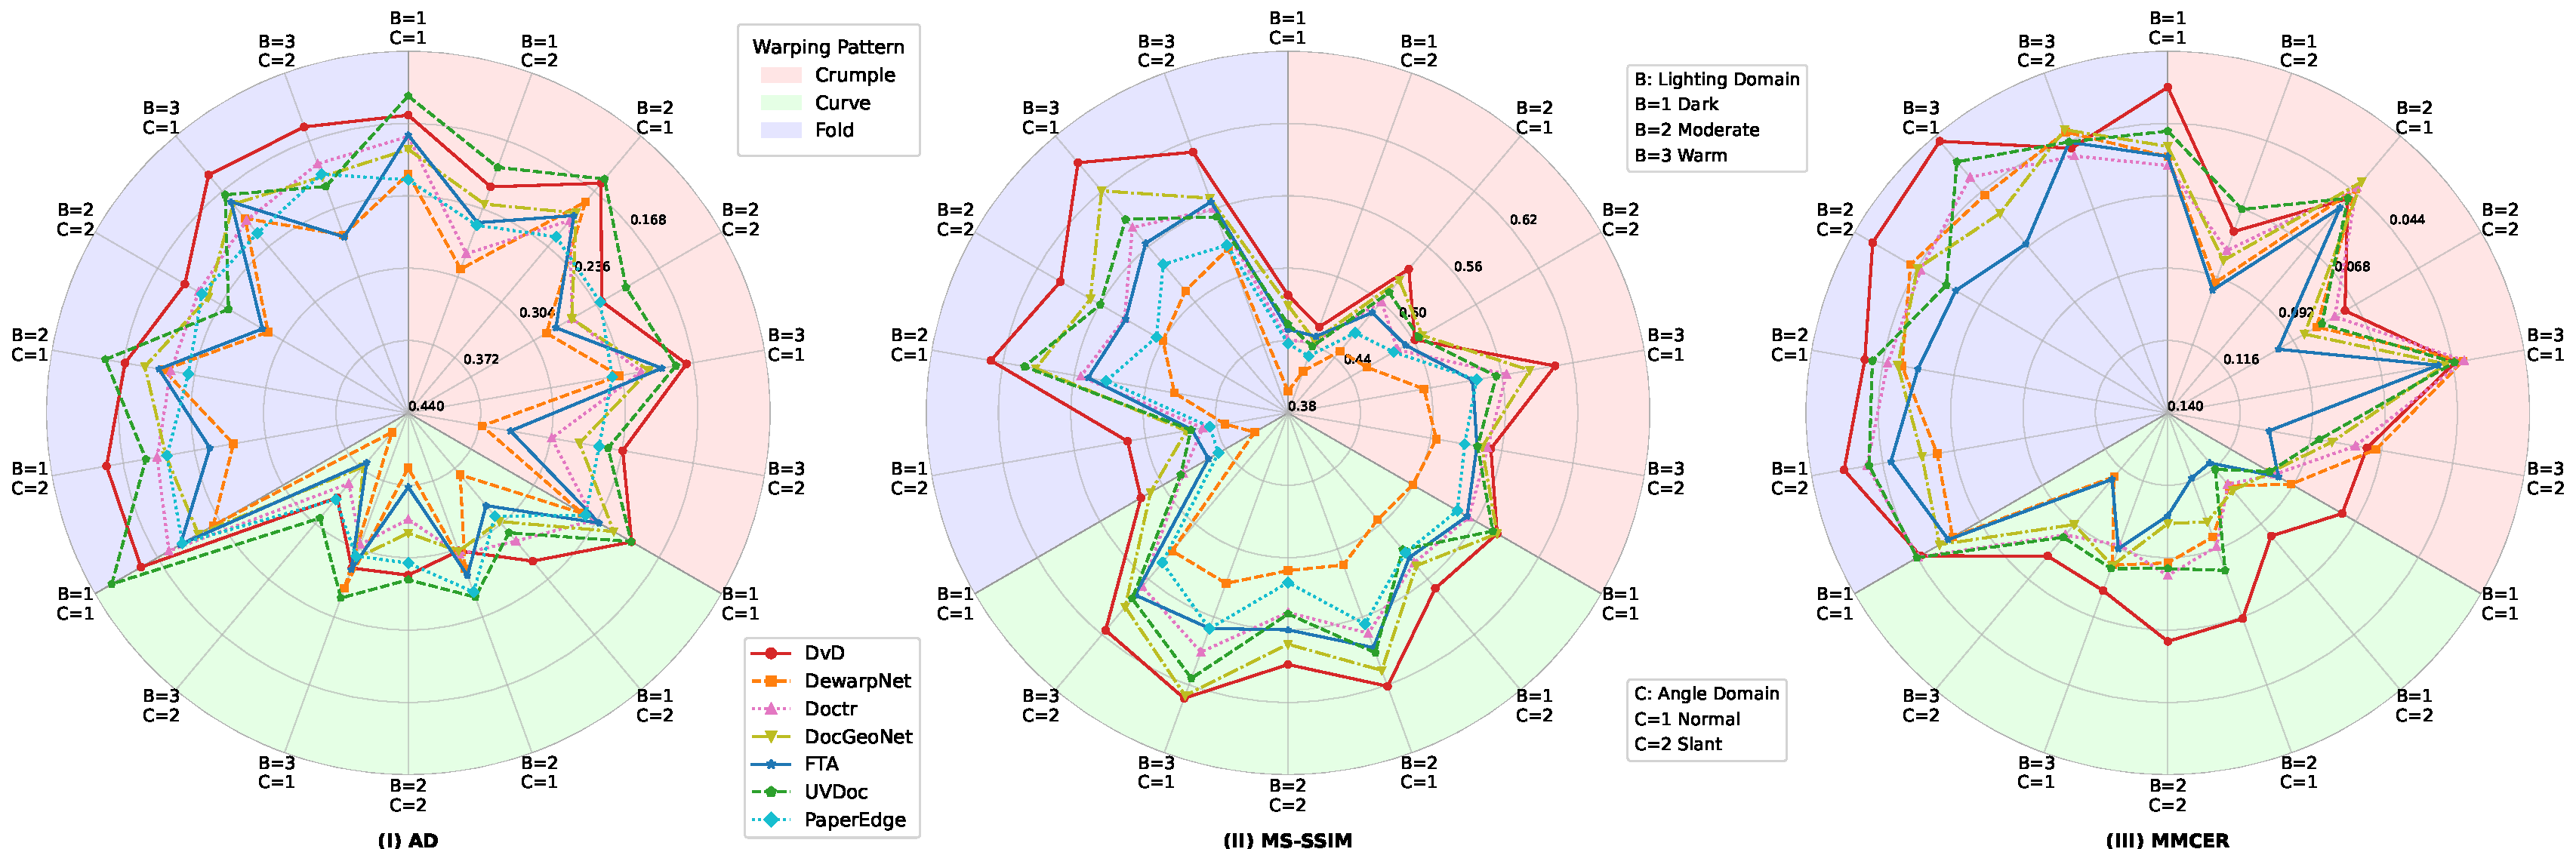
\includegraphics[width=0.95\linewidth]{figures/combined_radars_f1.pdf}
	\caption{More Quantitative dewarping performance comparisons on the \hbox{AnyPhotoDoc6600} benchmark dataset. Under the fixed "Single-column Paper" Layout Pattern, we provided 18 dimensions of evaluation for AD, MS-SSIM, and MMCER. }
\label{fig:vis_comparison2}
\end{figure*}
\begin{figure*}[tp]
	\centering
	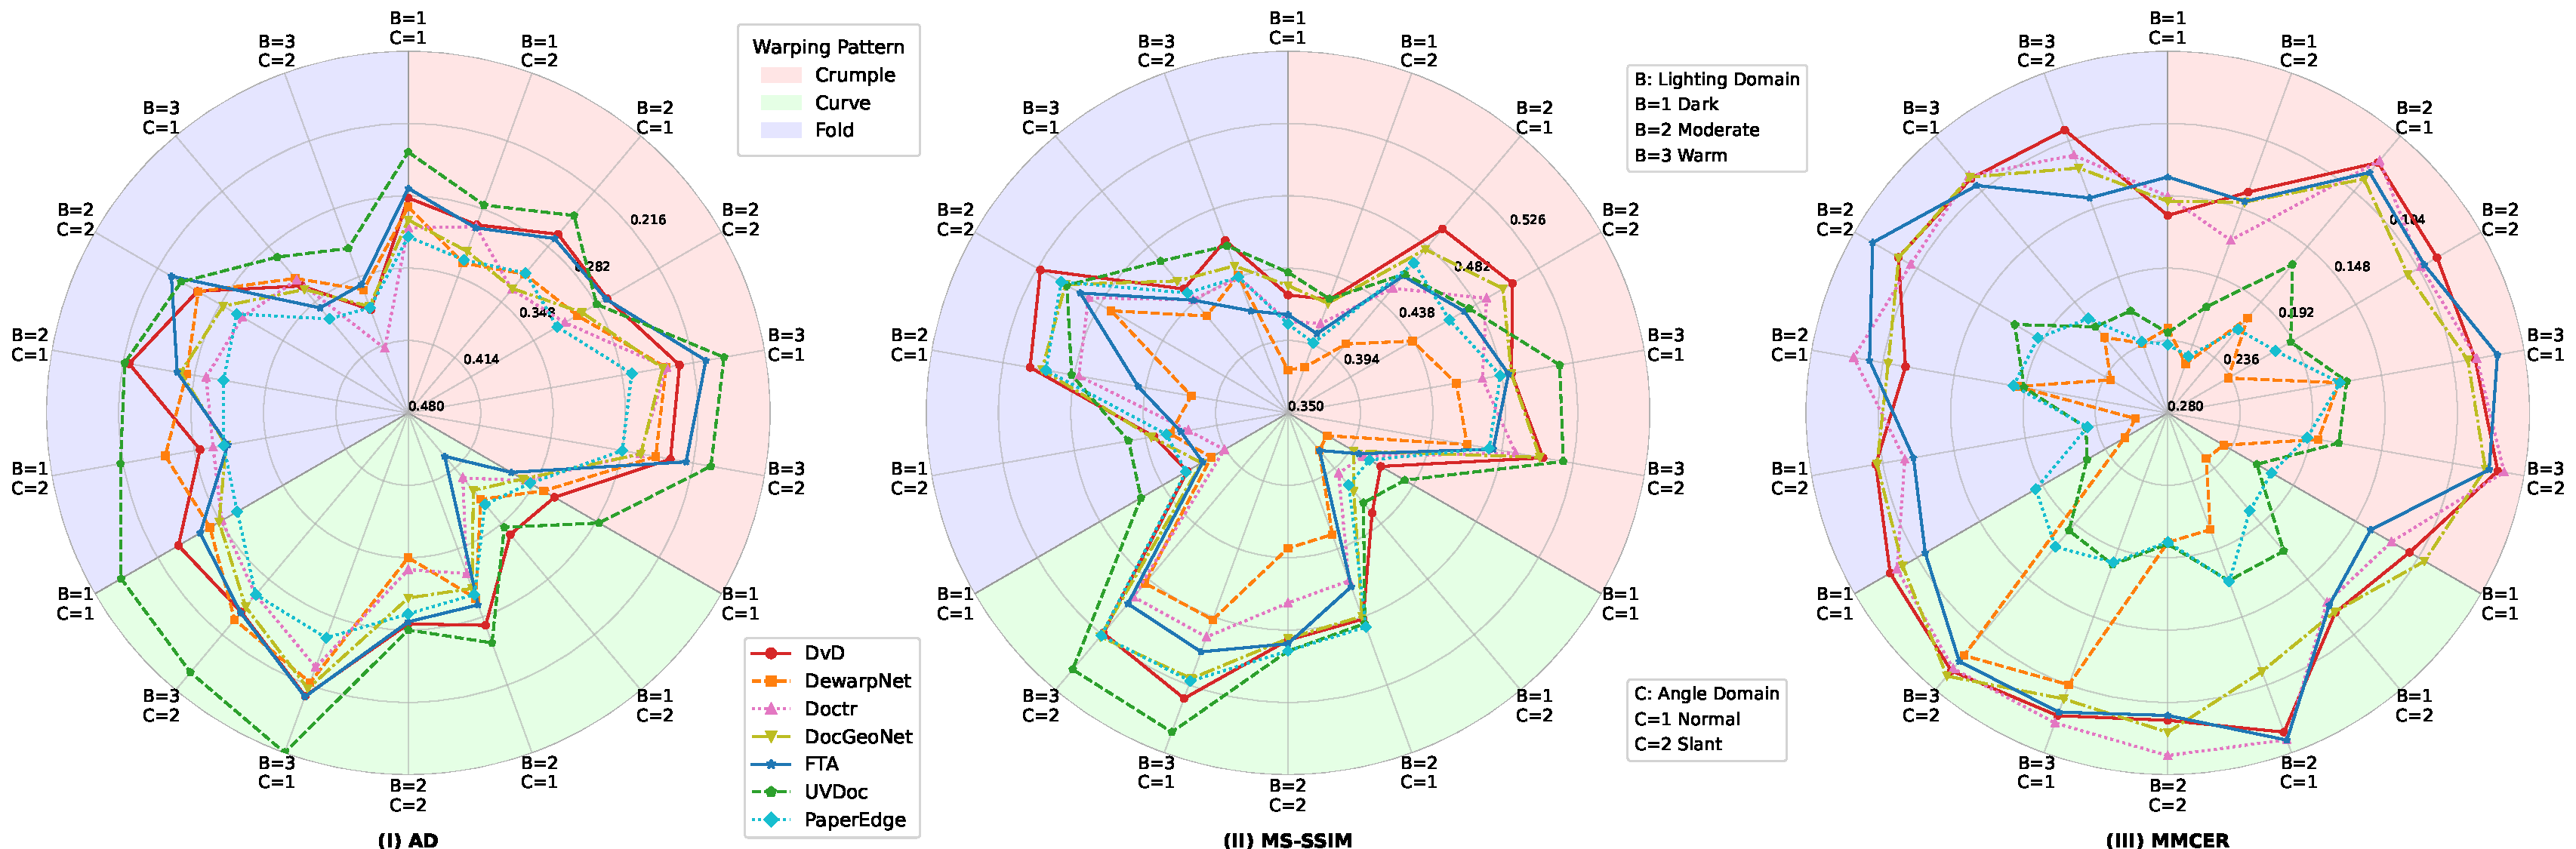
\includegraphics[width=0.95\linewidth]{figures/combined_radars_f7.pdf}
	\caption{More Quantitative dewarping performance comparisons on the \hbox{AnyPhotoDoc6600} benchmark dataset. Under the fixed "Magazine" Layout Pattern, we provided 18 dimensions of evaluation for AD, MS-SSIM, and MMCER.}
\label{fig:vis_comparison3}
\end{figure*}



\newpage
\bibliographystyle{ACM-Reference-Format}
\bibliography{reference}







% DO NOT INCLUDE ACKNOWLEDGMENTS IN AN ANONYMOUS SUBMISSION TO SIGGRAPH 2019








% \section{Limitation}
% 没时间写了








% end
% #####################################################################


% \textbf{(3) Sampling flexibility enables training-free templates-based dewarping}: Whereas discriminative paradigms applying deterministic point estimation are prone to obtain a fixed suboptimal prediction, DvD relies on distribution learning to enable flexibly sample multiple candidate flows that adhere to the real distribution of mapping. These candidate flows ensure the potential to cover optimal mapping. To screen out it, our DvD provides a post-processing module for optimal sample selection in the template-based dewarping~\cite{hertlein2023inv3d, hertlein2025docmatcher}. See Sect.~\ref{sec:method33}.
% Specifically, instead of training a cumbersome template-based dewarping model, we devise a training-free template-based scoring strategy to screen out the optimal mapping from multiple candidate mapping. 
% makes full use of the property from the diffusion model
% presuppose real mapping following a single peak distribution(uni-modal distribution), DvD unleashes this constraint, inherently allowing a more complex multi-modal distribution learning for mapping. 
% To the best of our knowledge, AnyPhotoDoc7000 is the most comprehensive dewarping benchmark up to now.




% \begin{table*}[t]
% \centering
% \caption{Revisiting currents document dewarping concerning working paradigm and task modeling essence. $y$ denotes model inputs(e.g., warped document images, text lines etc.), and $x$ symbolizes the deformation representation of warped document(e.g., mapping, backward mapping, forward mapping, etc.)  }
% \resizebox{0.95\linewidth}{!}{
% \begin{tabular}{lllc}
% \toprule
% \textbf{Periods} &\textbf{Paradigms Taxonomy}    & \textbf{Task Modeling Essence} & \textbf{Notes} \\ \midrule
% \multirow{1}{*}{Model-based} &Hand-crafted reconstruct-then-dewarp &$I_0=\mathcal{T}_\theta(\mathcal{R}_\theta(I_w))$ & Reconstruction $\mathcal{R}$ and transformation $\mathcal{T}$
% % \\&&$\mathcal{T}= \{GCS,DS,contents\}$ & where $\theta$ represent the parameter of $T_\theta$.  \\ 
% % &\multirow{2}{*}{Assumption-free} & \multirow{2}{*}{$x=T(y)$}        & Point-wise transformation $T$ is captured 
% % \\ &&&by special hardware device.
% \\
% \midrule
% \multirow{4.5}{*}{Learning-based} &\multirow{2}{*}{Previous discriminative paradigms}     & \multirow{1}{*}{$m = argmax_z p_\theta (f|I_w)$}    & Point(Mean) estimation for \\
% &&$I_0 = T_{m}(f)$& $p_\theta(f)$\\ \cmidrule(l){2-4} 
% &\multirow{2}{*}{Our generative paradigm~(DvD)}        &\multirow{1}{*}{$m = argmax_f p_\theta(f_{t-1} |f_t, f_0, I_w)$ }   & Distribution learning for       \\
% &&$I_0 = T_{m}(f)$& $p_\theta(f_0)$\\\bottomrule
% \end{tabular}}
% \label{tab:tab1}
% \end{table*}











% To address these limitations, for the first time, we explore a generative framework to explicitly maximize the conditional posterior probability of mapping $m$, i.e., ${\mathrm{argmax}}_{f} p(f|c_t)$. Unlike previous data-driven approaches, we achieve this by employing a conditional denoising diffusion model that jointly learns the \textit{likelihood} and \textit{prior} term through optimization of the following objective:
% \begin{equation}
% \begin{split}
%     f^{*} 
%     &= \mathcal{\epsilon}_\theta(c_t)\approx \underset{f}{\mathrm{argmax}}\  p(f|c_t)\\
%     &= \underset{f}{\mathrm{argmax}}\{
% \underbrace{\log p(c_t|f)}_{\textrm{likelihood term}}
% +\underbrace{\log p(f)}_{\textrm{prior term}}
% \},
% \end{split}
% \end{equation}



% Recent data-driven methods~\cite{ma2018docunet,das2019dewarpnet, xie2021document, jiang2022RDGR} have adopted deep neural networks $\mathcal{\epsilon}(\cdot)$ to directly approximate the \textit{likelihood} term, i.e., ${\mathrm{argmax}}_{f} \log p(c|f)$, without explicitly modeling the \textit{prior} term. In this formulation, $c$ consists of all kinds of feature descriptors related to the input image $I_d$.
% For example, DocGeoNet~\cite{Feng2022geodocnet} and FTA~\cite{li2023foreground} firstly extract the feature descriptors $c$, including text lines feature $l$, foreground feature $m$ and image feature $d$, and then regresses the mapping $m^{*}$ by vision transformer(ViT)~\cite{Dosovitskiy2021vit}:
% \begin{equation}
% f^{*} = \mathcal{\epsilon}_\theta(c)
% \approx \underset{f}{\mathrm{argmax}}\ \underbrace{\log p(c|f)}_{\textrm{data term}},
% \end{equation}
% where $\mathcal{\epsilon}_\theta(\cdot)$ and $\theta$ represent a neural networks and its parameters, respectively. 

% Compared to traditional methods~\cite{RN13,RN17,RN19,RN11} that suffer from poor generalization due to their reliance on hand-crafted priors, these recent data-driven methods omit explicit prior design and instead rely on large-scale datasets to implicitly learn the manifold of mappings. Despite demonstrating significant improvements in performance and generalization capability, they still struggle to deliver satisfactory results in the real world. We argue it stems from their neglect to explicitly model priors, which consequently constrains their ability to learn the optimal manifold of mappings.





% While the document dewarping task has been widely studied over two decades and empirically produce significant progress~\cite{RN58, verhoeven2023neural, li2023ladoc, jiaxin2022marior}, there is a lack of a theoretical perspective to consider document dewarping models. To fill this lack, we formulate a probabilistic perspective where we model the task as a posterior probability maximization problem using a Bayesian theory. In this probabilistic interpretation, the optimization objective for document dewarping can be defined with a likelihood term, measuring optimum mapping between warped and flat grids, and a prior term, encoding the manifold of mapping in the real world. 
% We argue that , without a theoretical foundation, analyzing this consequences of these choices is difficult.


% \begin{enumerate}[label=(\arabic*),leftmargin=*]
% \item We revisit the document dewarping task from a maximization of posterior probability formulation, critically analyzing the shortcomings of previous methods in either the likelihood term or the prior term. See Sect.~\ref{sec:method31}.
% \item Based on the formulation, we propose DvD, the first conditional diffusion framework tailored to jointly model both likelihood and prior terms. See Sect.~\ref{sec:method31}, \ref{sec:method32}.
% \item We theoretically attribute the previous content iteration mechanism to the learning of likelihood term, and thereby introduce a time-variant condition refinement mechanism for diffusion model, leading to more precise alignment of document content. See Sect.~\ref{sec:method31}, \ref{sec:method33}.
% \item Comprehensive experiments demonstrate state-of-the-art dewarping performance as well as the effectiveness of each component in our framework. See Sect.~\ref{sec:exp}.
% \end{enumerate}

%%%%%%%%%%%%%%%%%%%%%%%%%%%%%%%%%%%%%%%%%%%%%%%%%%%%%%%%%%

% these methods could be categorized into two branches:  methods and learning-based methods. 
% Document dewarping has been extensively studied through two primary approaches: traditional methods and learning-based techniques (see Table~\ref{tab:tab1}). 
% Numerous efforts have been undertaken to address the document dewarping task using either traditional methods or learning-based methods.

% However, such assumptions lead to limited generalization in real scenarios, and the dependence on hardware deviates from the user habits of using mobile phones to digitalize documents. 
% The early model-based methods~\cite{cao2003cylindrical, RN19, RN17} either utilize strong assumptions to devise some kind of transformations with limited generalization to warping patterns in real-world, or rely on special hardware to capture point-wise 3D transformations in an assumption-free manner whereas deviating from the user habit of using mobile phones to digitalize documents.

% In contrast, learning-based methods, pioneered by Ma et al.~\cite{ma2018docunet} in 2018 and further developed in~\cite{li2019document, das2019dewarpnet, RN7}, have emerged as the dominant paradigm due to their minimal reliance on explicit assumptions or specialized hardware. These methods typically adopt a discriminative approach based on pixel-wise regression, achieving state-of-the-art performance in recent works~\cite{RN58, verhoeven2023neural, li2023ladoc, yu_docreal_2024}. However, persistent challenges remain, including content misalignment artifacts and incomplete suppression of redundant backgrounds, as demonstrated in Fig.~\ref{fig:head_img} (b, b', c, c').
% Subsequent learning-based methods~\cite{ma2018docunet, li2019document, das2019dewarpnet} have shifted the paradigm from model-driven to data-driven, significantly lessening reliance on both assumptions and hardware. These learning-based methods commonly adopt a discriminative regression paradigm to predict pixel-wise mapping or mapping. Notwithstanding achieving state-of-the-art~\cite{verhoeven2023neural, li2023ladoc, yu_docreal_2024}, they still face unsatisfactory accuracy and poor generalization, hampering their availability in real-world scenarios.




% DocUNet~\cite{li2019document} pioneered an end-to-end deep learning approach for document dewarping by employing a stacked U-Net to directly predict a pixel-wise forward mapping from distorted to rectified document images. In contrast, ~\cite{das2019dewarpnet} introduces an explicit 3D representation by first regressing a 3D coordinate map of the document surface and then remapping the texture onto a flat plane. 

% Among the recent works, DocTr~\cite{feng2021doctr} leverages a Transformer architecture to capture long-range dependencies and directly predict pixel-wise mappings, thus effectively rectifying distorted document images. DDCP~\cite{xie2021document} employs a convolutional network to extract rich image features and uses a control point-based strategy to generate sparse mappings that are then interpolated into a complete distortion flow, offering a more flexible and efficient rectification mechanism. These approaches typically adopt a discriminative regression strategy where deep neural networks are trained end-to-end to directly infer the mapping relationship or distortion flow for each pixel, thereby bypassing the need for explicit 3D reconstruction and dedicated measurement equipment. Despite the high performance of these discriminative regression approaches under controlled, laboratory conditions, they still face challenges when applied to real-world images. 
% For instance, UVDoc~\cite{verhoeven2023neural} uses a lightweight convolutional neural network with a dual-head output—one head regresses a 3D mesh that encodes the document’s physical deformation, while the other predicts a 2D backward mapping grid for re-sampling—to correct distortions; in contrast, \cite{li2023ladoc} introduces a Transformer-based layout-aware network that integrates global UV mapping with local text-line information to achieve accurate pixel-level distortion flow regression; meanwhile, 
% DocReal~\cite{yu_docreal_2024} presents a robust, control-point-based framework that leverages an Enet module to suppress background noise and incorporates attention-enhanced control points (AECP) to precisely capture local deformations. When processing images with severe deformations and complex backgrounds, they still yield issues such as inaccurate document alignment and excessive background redundancy. 
% Moreover, a recent study~\cite{hertlein2025docmatcher} further suggests that incorporating additional structured information (e.g., an ideal flat template image) at inference time can supply powerful prior knowledge to enhance the dewarping process. However, this method highly relies on fixed prior structures, making it difficult to capture the complex distortions encountered in real-world environments. 



% Motivated by these findings, we propose a novel generative paradigm approach, \textbf{DvD}, which departs from the conventional discriminative regression framework by learning to generate mappings from Gaussian noise—thereby capturing a more flexible, multimodal representation of distortions and ultimately achieving a higher overall dewarping effect and improved robustness in real-world scenarios.




% To improve the regression accuracy, they primarily pursue three directions: the contribution of high-fidelity photographic document datasets or the advancement of document representation learning through enhanced visual feature extraction architectures and more sophisticated neural network designs.


% \begin{figure*}[htp]
% 	\centering
%      \setlength{\tabcolsep}{0.8pt}
%      \renewcommand{\arraystretch}{1}
% 	\begin{tabular}{cccccccc}
% 				\begin{tikzpicture}[
% 			baseline=(img.base),
% 			remember picture, % 允许后续通过 (pic cs:name) 引用坐标
% 			every node/.style={inner sep=0pt}
% 			]
% 			\node(img) {
% 				\includegraphics[width=0.122\linewidth,height=0.1674\linewidth]{figures/comparison/crop/7_1 copy.jpg}
% 			};
% 			\coordinate (pic) at (img.south west);
% 			\draw[red,thick, densely dotted] 
% 			($(pic) + ({0.7*0.122\linewidth}, {0.1*0.1674\linewidth})$) --
% 			($(pic) + ({0.7*0.122\linewidth}, {0.6*0.1674\linewidth})$);
% 		\end{tikzpicture} & 
% 		\includegraphics[width=0.12\linewidth,height=0.1674\linewidth]{figures/comparison/Marior/7_1.jpg} & 
%         \includegraphics[width=0.122\linewidth,height=0.1674\linewidth]{figures/comparison/UVDoc/7_1.jpg} &
%         \includegraphics[width=0.122\linewidth,height=0.1674\linewidth]{figures/comparison/LADoc/7_1_rec.jpg} &
%         \includegraphics[width=0.122\linewidth,height=0.1674\linewidth]{figures/comparison/FTA/7_1 copy.jpg} & 
%         \includegraphics[width=0.122\linewidth,height=0.1674\linewidth]{figures/comparison/docreal/7_1_rec.jpg} & 
%         \includegraphics[width=0.122\linewidth,height=0.1674\linewidth]{figures/comparison/gpt4o/7_1.jpg} & 
%         \includegraphics[width=0.122\linewidth,height=0.1674\linewidth]{figures/comparison/0428_1/warped_7_1 copy.jpg} \\
%         \includegraphics[width=0.122\linewidth,height=0.1674\linewidth]{figures/comparison/crop/49_1 copy.jpg} & 
%         \includegraphics[width=0.12\linewidth,height=0.1674\linewidth]{figures/comparison/Marior/49_1.jpg} & 
%         \includegraphics[width=0.122\linewidth,height=0.1674\linewidth]{figures/comparison/UVDoc/49_1.jpg} &
%         \includegraphics[width=0.122\linewidth,height=0.1674\linewidth]{figures/comparison/LADoc/49_1_rec.jpg} &
%         \includegraphics[width=0.122\linewidth,height=0.1674\linewidth]{figures/comparison/FTA/49_1 copy.jpg} & 
%         \includegraphics[width=0.122\linewidth,height=0.1674\linewidth]{figures/comparison/docreal/49_1_rec.jpg} & 
%         \includegraphics[width=0.122\linewidth,height=0.1674\linewidth]{figures/comparison/gpt4o/49_1.jpg} & 
%         \includegraphics[width=0.122\linewidth,height=0.1674\linewidth]{figures/comparison/0428_1/warped_49_1 copy.jpg} \\
% 		\includegraphics[width=0.122\linewidth,height=0.1674\linewidth]{figures/comparison/crop/64_2 copy.jpg} & 
% 		\includegraphics[width=0.12\linewidth,height=0.1674\linewidth]{figures/comparison/Marior/64_2.jpg} & 
% 		\includegraphics[width=0.122\linewidth,height=0.1674\linewidth]{figures/comparison/UVDoc/64_2.jpg} &
% 		\includegraphics[width=0.122\linewidth,height=0.1674\linewidth]{figures/comparison/LADoc/64_2_rec.jpg} &
% 		\includegraphics[width=0.122\linewidth,height=0.1674\linewidth]{figures/comparison/FTA/64_2 copy.jpg} & 
% 		\includegraphics[width=0.122\linewidth,height=0.1674\linewidth]{figures/comparison/docreal/64_2_rec.jpg} & 
% 		\includegraphics[width=0.122\linewidth,height=0.1674\linewidth]{figures/comparison/gpt4o/64_2.jpg} & 
% 		\includegraphics[width=0.122\linewidth,height=0.1674\linewidth]{figures/comparison/0428_1/warped_64_2 copy.jpg} \\
%         \\[-16pt]
%         \scriptsize Input &
%         \scriptsize \cite{jiaxin2022marior} &
%         \scriptsize  \cite{verhoeven2023neural} &
%         \scriptsize \cite{li2023ladoc} &
%         \scriptsize \cite{li2023foreground} &
%         \scriptsize \cite{yu_docreal_2024} &
%         \scriptsize GPT-4o &
%         \scriptsize ours \\
% 	\end{tabular}
% 	\caption{Qualitative comparisons on the DocUNet benchmark. From left to right: input, DewarpNet, DocTr, FDRNet, PaperEdge, Marior, DocGeoNet, ours. \label{fig:vis_compa1}}
% \end{figure*}



% \begin{figure*}[htp]
% 	\centering
% 	\setlength{\tabcolsep}{0.8pt}
% 	\renewcommand{\arraystretch}{1}
% 	\begin{tabular}{cccccccc}
% 		\begin{tikzpicture}[
% 			baseline=(img.base),
% 			remember picture, % 允许后续通过 (pic cs:name) 引用坐标
% 			every node/.style={inner sep=0pt}
% 			]
% 			\node(img) {
% 				\includegraphics[width=0.122\linewidth,height=0.1674\linewidth]{figures/comparison/crop/6_1 copy.jpg}
% 			};
% 			\coordinate (pic) at (img.south west);
% 			\draw[red,thick, densely dotted] 
% 			($(pic) + ({0.7*0.122\linewidth}, {0.1*0.1674\linewidth})$) --
% 			($(pic) + ({0.7*0.122\linewidth}, {0.6*0.1674\linewidth})$);
% 		\end{tikzpicture} & 
% 		\includegraphics[width=0.12\linewidth,height=0.1674\linewidth]{figures/comparison/Marior/6_1.jpg} & 
% 		\includegraphics[width=0.122\linewidth,height=0.1674\linewidth]{figures/comparison/UVDoc/6_1.jpg} &
% 		\includegraphics[width=0.122\linewidth,height=0.1674\linewidth]{figures/comparison/LADoc/6_1_rec.jpg} &
% 		\includegraphics[width=0.122\linewidth,height=0.1674\linewidth]{figures/comparison/FTA/6_1 copy.jpg} & 
% 		\includegraphics[width=0.122\linewidth,height=0.1674\linewidth]{figures/comparison/docreal/6_1_rec.jpg} & 
% 		\includegraphics[width=0.122\linewidth,height=0.1674\linewidth]{figures/comparison/0428_1/warped_6_1 copy.jpg} & 
% 		\includegraphics[width=0.122\linewidth,height=0.1674\linewidth]{figures/comparison/gpt4o/6_1.jpg} \\
% 		\includegraphics[width=0.122\linewidth,height=0.1674\linewidth]{figures/comparison/crop/16_1 copy.jpg} & 
% 		\includegraphics[width=0.12\linewidth,height=0.1674\linewidth]{figures/comparison/Marior/16_1.jpg} & 
% 		\includegraphics[width=0.122\linewidth,height=0.1674\linewidth]{figures/comparison/UVDoc/16_1.jpg} &
% 		\includegraphics[width=0.122\linewidth,height=0.1674\linewidth]{figures/comparison/LADoc/16_1_rec.jpg} &
% 		\includegraphics[width=0.122\linewidth,height=0.1674\linewidth]{figures/comparison/FTA/16_1 copy.jpg} & 
% 		\includegraphics[width=0.122\linewidth,height=0.1674\linewidth]{figures/comparison/docreal/16_1_rec.jpg} & 
% 		\includegraphics[width=0.122\linewidth,height=0.1674\linewidth]{figures/comparison/gpt4o/16_1.jpg} & 
% 		\includegraphics[width=0.122\linewidth,height=0.1674\linewidth]{figures/comparison/0428_1/warped_16_1 copy.jpg} \\
% 		\includegraphics[width=0.122\linewidth,height=0.1674\linewidth]{figures/comparison/crop/60_1 copy.jpg} & 
% 		\includegraphics[width=0.12\linewidth,height=0.1674\linewidth]{figures/comparison/Marior/60_1.jpg} & 
% 		\includegraphics[width=0.122\linewidth,height=0.1674\linewidth]{figures/comparison/UVDoc/60_1.jpg} &
% 		\includegraphics[width=0.122\linewidth,height=0.1674\linewidth]{figures/comparison/LADoc/60_1_rec.jpg} &
% 		\includegraphics[width=0.122\linewidth,height=0.1674\linewidth]{figures/comparison/FTA/60_1 copy.jpg} & 
% 		\includegraphics[width=0.122\linewidth,height=0.1674\linewidth]{figures/comparison/docreal/60_1_rec.jpg} & 
% 		\includegraphics[width=0.122\linewidth,height=0.1674\linewidth]{figures/comparison/gpt4o/60_1.jpg} & 
% 		\includegraphics[width=0.122\linewidth,height=0.1674\linewidth]{figures/comparison/0428_1/warped_60_1 copy.jpg} \\
% 		\\[-16pt]
% 		\scriptsize Input &
% 		\scriptsize \cite{jiaxin2022marior} &
% 		\scriptsize  \cite{verhoeven2023neural} &
% 		\scriptsize \cite{li2023ladoc} &
% 		\scriptsize \cite{li2023foreground} &
% 		\scriptsize \cite{yu_docreal_2024} &
% 		\scriptsize GPT-4o &
% 		\scriptsize ours \\
% 	\end{tabular}
% 	\caption{Qualitative comparisons on the DocUNet benchmark. From left to right: input, DewarpNet, DocTr, FDRNet, PaperEdge, Marior, DocGeoNet, ours. \label{fig:vis_compa2}}
% \end{figure*}




% Witnessing the superior progress of multimodal large language models (MLLMs) in OCR capabilities recently~\cite{wei2024general, karmanov_eclair_2025, nassar_smoldocling_2025}, we identify that there is no exploration about whether document dewarping is still useful for OCR using multimodal large-language models(MLLMs). To fill the blank


% \textbf{(2) Distribution learning boosts better generalization}: Distinct from the discriminative paradigm that implicitly captures data distribution, DvD inherently understands the distribution of mapping by learning to generate it. This property allows DvD to capture a more complex mapping in the real world, consequently boosting better generalization. 
